%
\documentclass[10pt,twocolumn,letterpaper]{article}

\usepackage{cvpr}
\usepackage{times}
\usepackage{epsfig}
\usepackage{graphicx}
\usepackage{amsmath}
\usepackage{amssymb}
\usepackage{multirow}
\usepackage{longtable}
\usepackage{lipsum}
\usepackage[table,xcdraw]{xcolor}

% Include other packages here, before hyperref.
\newcommand{\rak}[1]{{\color{red}{rak: #1}}}
\newcommand{\ma}[1]{{\color{purple}{ma: #1}}}
\newcommand{\mgm}[1]{{\color{cyan}{mgm: #1}}}

\definecolor{objectColor}{rgb}{0.8, 0.254, 0.145}
\newcommand{\object}[1]{{\color{objectColor}{#1}}}
\definecolor{relationshipColor}{rgb}{0.415, 0.658, 0.309}
\newcommand{\relationship}[1]{{\color{relationshipColor}{#1}}}
\definecolor{actionColor}{rgb}{0.964, 0.698, 0.419}
\newcommand{\action}[1]{{\color{actionColor}{#1}}}
\definecolor{timeColor}{rgb}{0.403, 0.305, 0.654}
\newcommand{\temporal}[1]{{\color{timeColor}{#1}}}

% If you comment hyperref and then uncomment it, you should delete
% egpaper.aux before re-running latex.  (Or just hit 'q' on the first latex
% run, let it finish, and you should be clear).
\usepackage[breaklinks=true,bookmarks=false]{hyperref}

% \cvprfinalcopy % *** Uncomment this line for the final submission

\def\cvprPaperID{2764} % *** Enter the CVPR Paper ID here
\def\httilde{\mbox{\tt\raisebox{-.5ex}{\symbol{126}}}}

% Pages are numbered in submission mode, and unnumbered in camera-ready
%\ifcvprfinal\pagestyle{empty}\fi
\setcounter{page}{4321}
\begin{document}

%%%%%%%%% TITLE
\title{Action Genome Question Answers: \\ A Benchmark for Compositional Spatio-Temporal Reasoning in Videos}

\author{Madeleine Grunde-McLaughlin\\
University of Pennsylvania\\
%Philadelphia, Pennsylvania\\
{\tt\small madeleine.grunde@gmail.com}

\and
Ranjay Krishna\\
Stanford University\\
%Palo Alto, California\\
{\tt\small ranjay.krishna@gmail.com}

\and
Maneesh Agrawala\\
Stanford University\\
%Palo Alto, California\\
{\tt\small maneesh@cs.stanford.edu}


}
\maketitle
\pagestyle{empty}

%%%%%%%%% ABSTRACT
\begin{abstract}
Our visual perception is characterized by spatio-temporal compositionality, allowing us to comprehend visual events as a composition of actions involving actors interacting with objects. While training vision models to exhibit such compositionality has been a long standing goal in Computer Vision, existing video benchmarks only test simple temporal logic. 
We build a pipeline to programmatically generate a benchmark by combining Action Genome's spatio-temporal scene graph annotations with handcrafted templates and programs.
With the pipeline, we introduce AGQA: a benchmark for compositional spatio-temporal reasoning. Utilizing language as the medium to test for spatio-temporal compositionality, AGQA presents $1.77M$ balanced and $133M$ unbalanced question answer pairs for $9.6K$ videos, which is orders of magnitude larger than existing benchmarks.
AGQA tests a wide variety of spatio-temporal reasoning skills, including action sequencing, temporal localization, human-object interaction recognition, length, repetition, and compositional reasoning.
Using AGQA, we evaluate modern visual reasoning systems, demonstrating that the best video question answering models barely perform better than non-visual baselines exploiting linguistic bias. Although some models generalize to longer video inputs, none of them generalize to novel compositions unseen during training.
\end{abstract}

%%%%%%%%% BODY TEXT

\section{Introduction}
The ability to perceive and reason about the world's actors, actions, objects, and relationships has been a longstanding goal for Computer Vision. 
Traditionally, we have benchmarked progress towards this goal using tasks like visual question answering~\cite{antol2015vqa}, in which a model's reasoning skills are evaluated by it's ability to answer questions about visual stimuli. 
A variety of benchmarks have been created to test a model's capabilities at answering questions about images~\cite{johnson2017clevr,hudson2019gqa,antol2015vqa,zellers2019recognition,goyal2017making,krishna2017visual,zhu2016visual7w,kim2020answering} and about videos~\cite{tapaswi2016movieqa,lei2018tvqa,jang2017tgif,kim2017deepstory,xu2017video,maharaj2017dataset,zeng2016leveraging,yu2019activitynet, yi2019clevrer, mun2017marioqa}. 
Ideally, models trained on these benchmarks should be capable of reasoning over both spatial relationships between objects~\cite{krishna2017visual,lu2016visual} and temporal ordering of actions~\cite{zacks2001events,ji2020action}. 
Unfortunately, since most question-answering benchmarks operate over images, they are limited to only testing spatial relationships (e.g.~"What is on top of the table?")~\cite{hudson2019gqa,krishna2017visual,antol2015vqa} or at most guessing common sense events occurring before and after the image~\cite{park2020visualcomet,zellers2019recognition}. 
The few existing video benchmarks have questions only use simple temporal logic (e.g."What does the bear on right do after sitting?")~\cite{jang2017tgif,xu2017video,maharaj2017dataset,zeng2016leveraging,yu2019activitynet}. 
However, to answer questions that require models to jointly compose spatial and temporal reasoning in more complex questions (e.g."What did they do to the last object they put down before opening the window?"), we need newer benchmarks and a new class of models.


\begin{figure}[t]
    \centering
    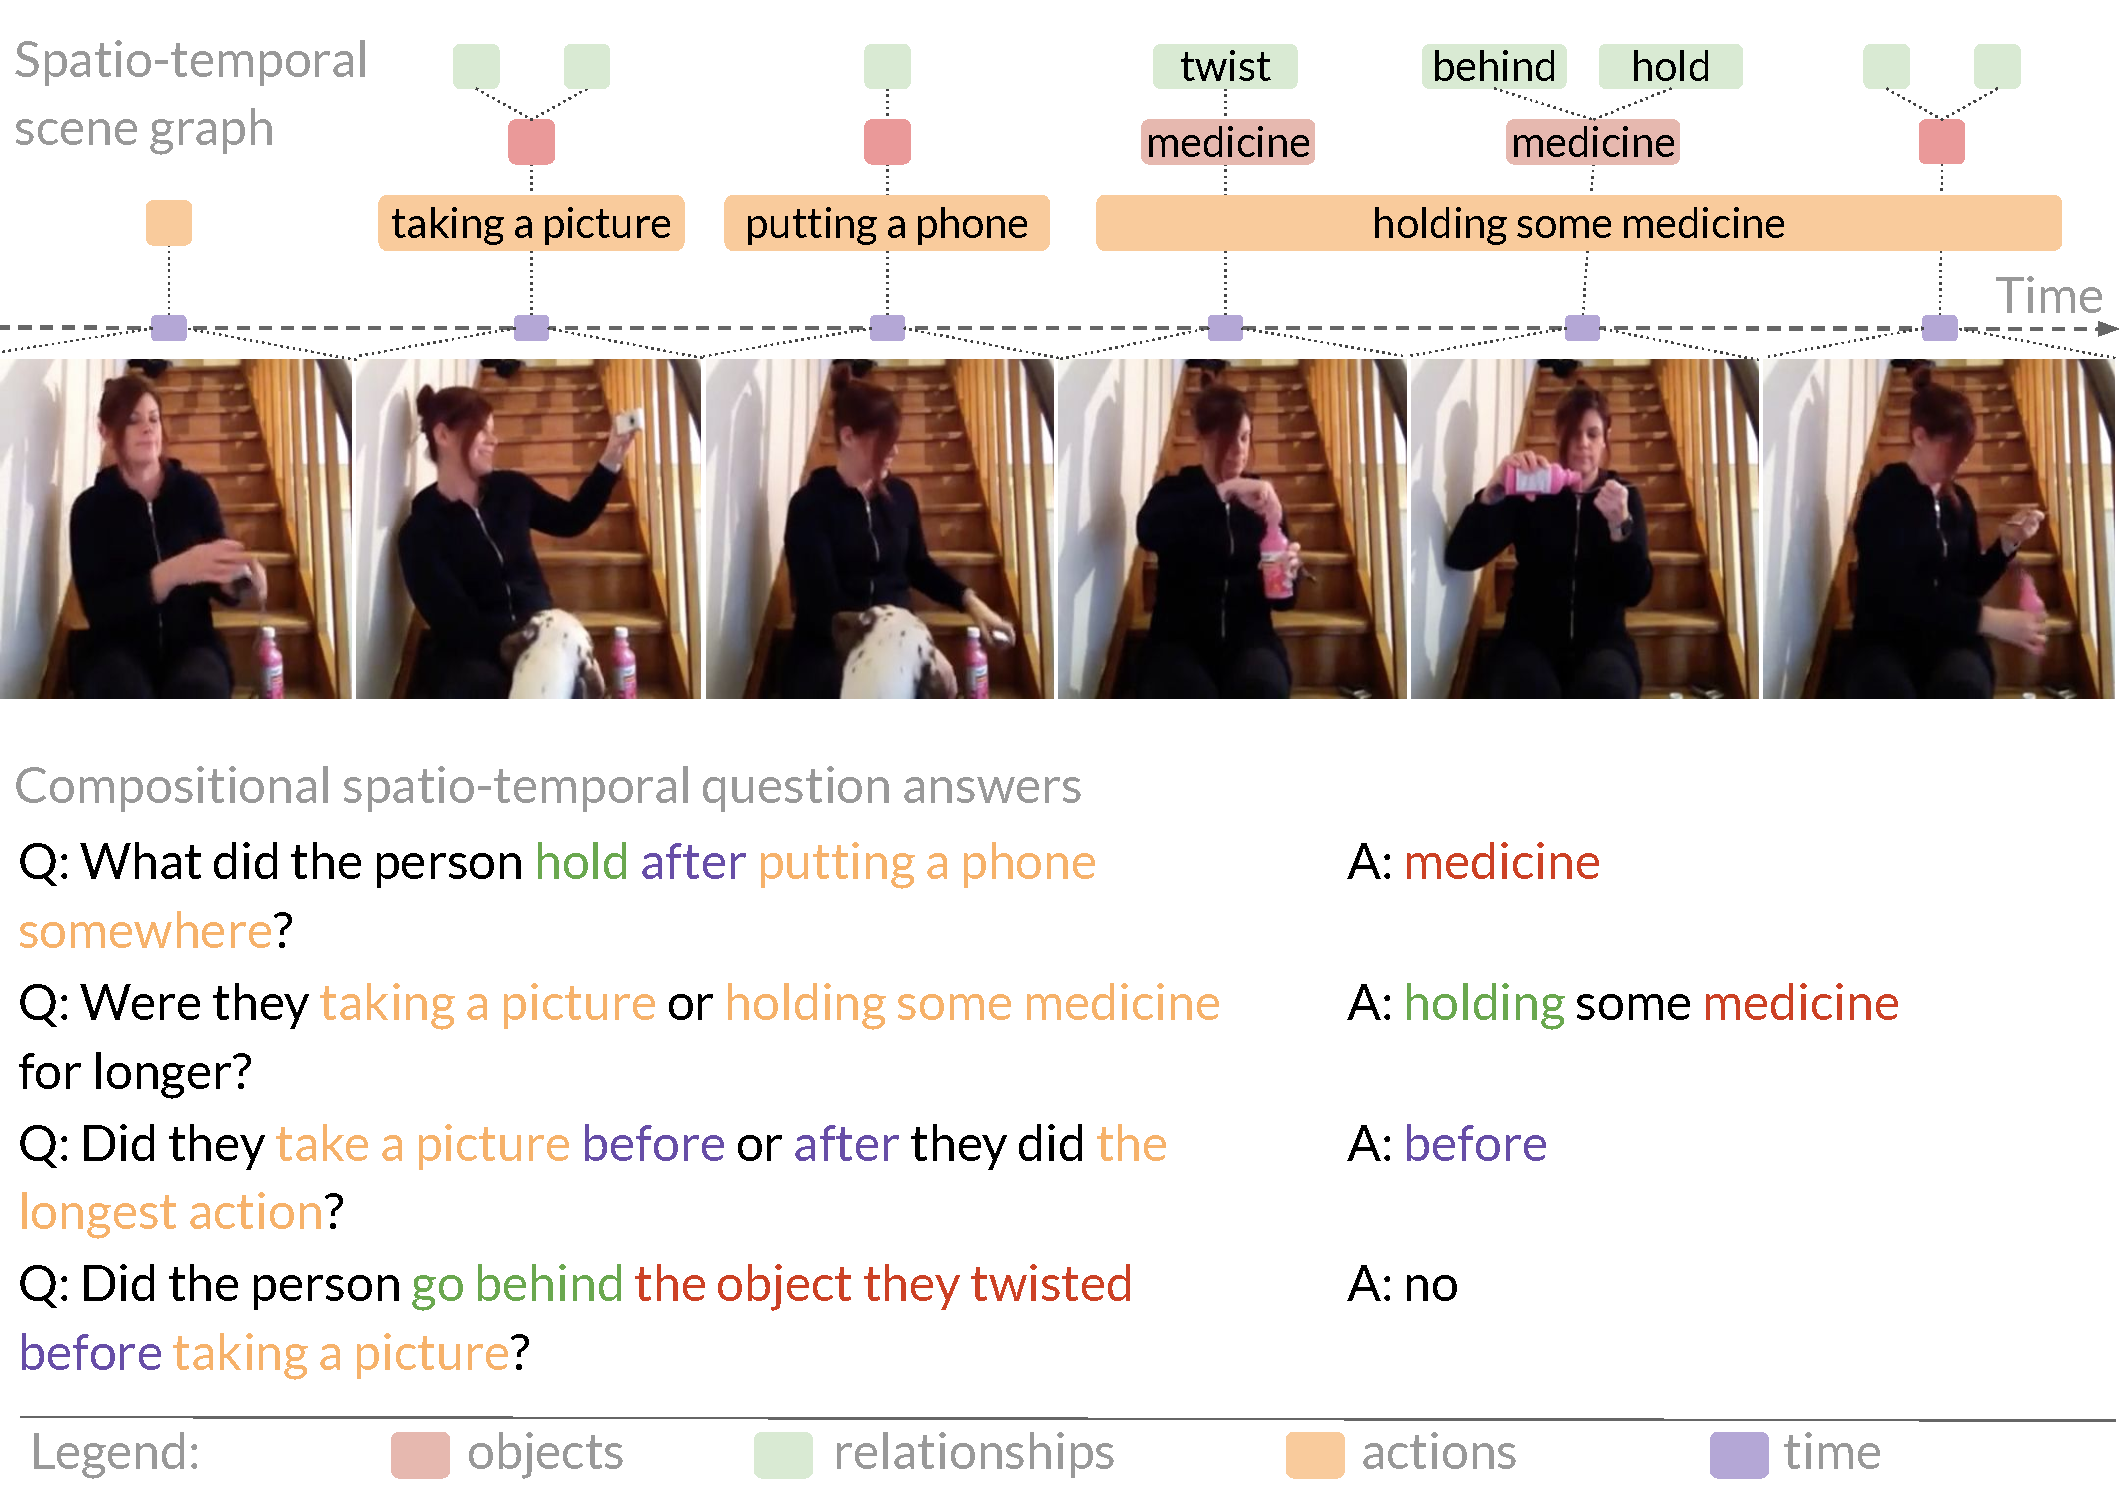
\includegraphics[width=\columnwidth]{figures/pull.pdf}
    \caption{We introduce AGQA: a new benchmark to test for compositional spatio-temporal reasoning. AGQA contains a balanced benchmark of 1.77M question answer pairs associated with 10K videos and an unbalanced set of 133M question answers in total. We argue that existing benchmarks do not test for compositional spatio-temporal reasoning and find that existing video question answering models do not demonstrate compositional capability.}
    \label{fig:pull}
\end{figure}

Meanwhile, Cognitive Science postulates that people actively encode events into structures characterized by systematic compositionality~\cite{michotte2017perception,barker1951one,zacks2001perceiving} --- the algebraic ability to comprehend a combinatorial number of novel combinations from known components. Once we learn to identify objects like \object{medicine}, understand relationships like \relationship{holding}, and recognize actions like \action{putting a phone somewhere}, we can compose these ideas together to explain when someone is \relationship{holding} \object{medicine} \temporal{before} \action{putting a phone somewhere}  (Figure~\ref{fig:pull}). This compositional ability is reflected in the language we use to communicate with one another~\cite{chomsky2002syntactic,montague1970universal}, allowing us the ability to showcase compositional reasoning and generate tests to check for this ability. We can ask questions like ``What did the person \relationship{hold} \temporal{after} \action{putting a phone somewhere}?'' and expect someone capable of spatio-temporal compositional reasoning to answer ``\object{medicine}''. While
that was a relatively simple composition, more complex questions can involve reasoning over novel combinations of many different types of objects, relationships, and actions. So while such compositional behavior seems fundamental to developing vision models that can reason over events in the world, we have developed compositional benchmarks using state images~\cite{hudson2019gqa} or synthetic worlds~\cite{lake2018generalization,yi2019clevrer} which either are not spatio-temporal or do not reflect the diversity of real-world events.

Creating a benchmark for spatio-temporal questions is a challenging endeavor. It requires (1) identifying the core primitives that can be composed together, (2) be diverse enough to reflect a variety of real world events, (3) be minimally biased to prevent simple solutions, and (4) be capable of testing a variety of compositional metrics. 
Questions automatically generated from video captions often lack diversity in structure~\cite{yu2019activitynet,jang2017tgif}, while human annotations are too expensive to get a large enough sample devoid of biases in language or concepts~\cite{zeng2016leveraging,yu2019activitynet}. Additionally, generating a benchmark that allows us to test compositional behavior must contain a training\/test split where particular compositions only occur in the test set. Producing annotation workflows to adhere to such explicit splits requires premeditated planning, tedious verification and is largely unexplored in the crowdsourcing literature.

We introduce the Action Genome Question Answering (AGQA), a new benchmark for compositional spatio-temporal reasoning. \rak{TODO: working on this paragraph. The next couple of sentences are just random. ignore them}
To achieve these goals, we developed an automatic approach that converts Action Genome’s spatio-temporal scene graphs, containing objects, relationships, actors, and actions, into highly complex questions~\cite{ji2020action}. This process gives us tight control over the content of the questions to create a suite of metrics measuring individual spatio-temporal reasoning skills and compositional reasoning skills. We test AGQA on state-of-the art models to evaluate their strengths and weaknesses. 
By recursively generating questions with direct references, indirect references, and temporal localizations, our question generation pipeline creates a diverse set of questions that can be trained and tested all together or separated by type.


AGQA presents a balanced benchmark of $1.77$ million question answer pairs associated with $10K$ videos, along with an additional unbalanced set of $133M$ question answer pairs for future work to utilize. Each question is associated with a corresponding program, outlining the necessary visual reasoning steps requires to answer the question (Figure~\ref{fig:tree} \rak{Add in the figure with the question steps outlined here.}). These reasoning steps involve identifying objects, understanding relationships and recognizing actions, which are each spatio-temporally grounded in the videos, using Action Genome~\cite{ji2020action}. AGQA contains multiple training and test splits, each testing for different forms of compositionality. These split tests how well models generalize to novel compositions they have not seen during training, or to videos longer than the ones in the training set or to questions with more compositional steps. Using AGQA, we evaluate modern visual reasoning systems~\cite{}, and find that the best model~\cite{} barely performs better than random chance of and it's improvements are largely due to exploiting language bias. We also find that while some models are able to generalize to videos of longer length, all of them are unable to generalize to questions with novel compositions unseen during training.

\begin{figure}[t]
    \centering
    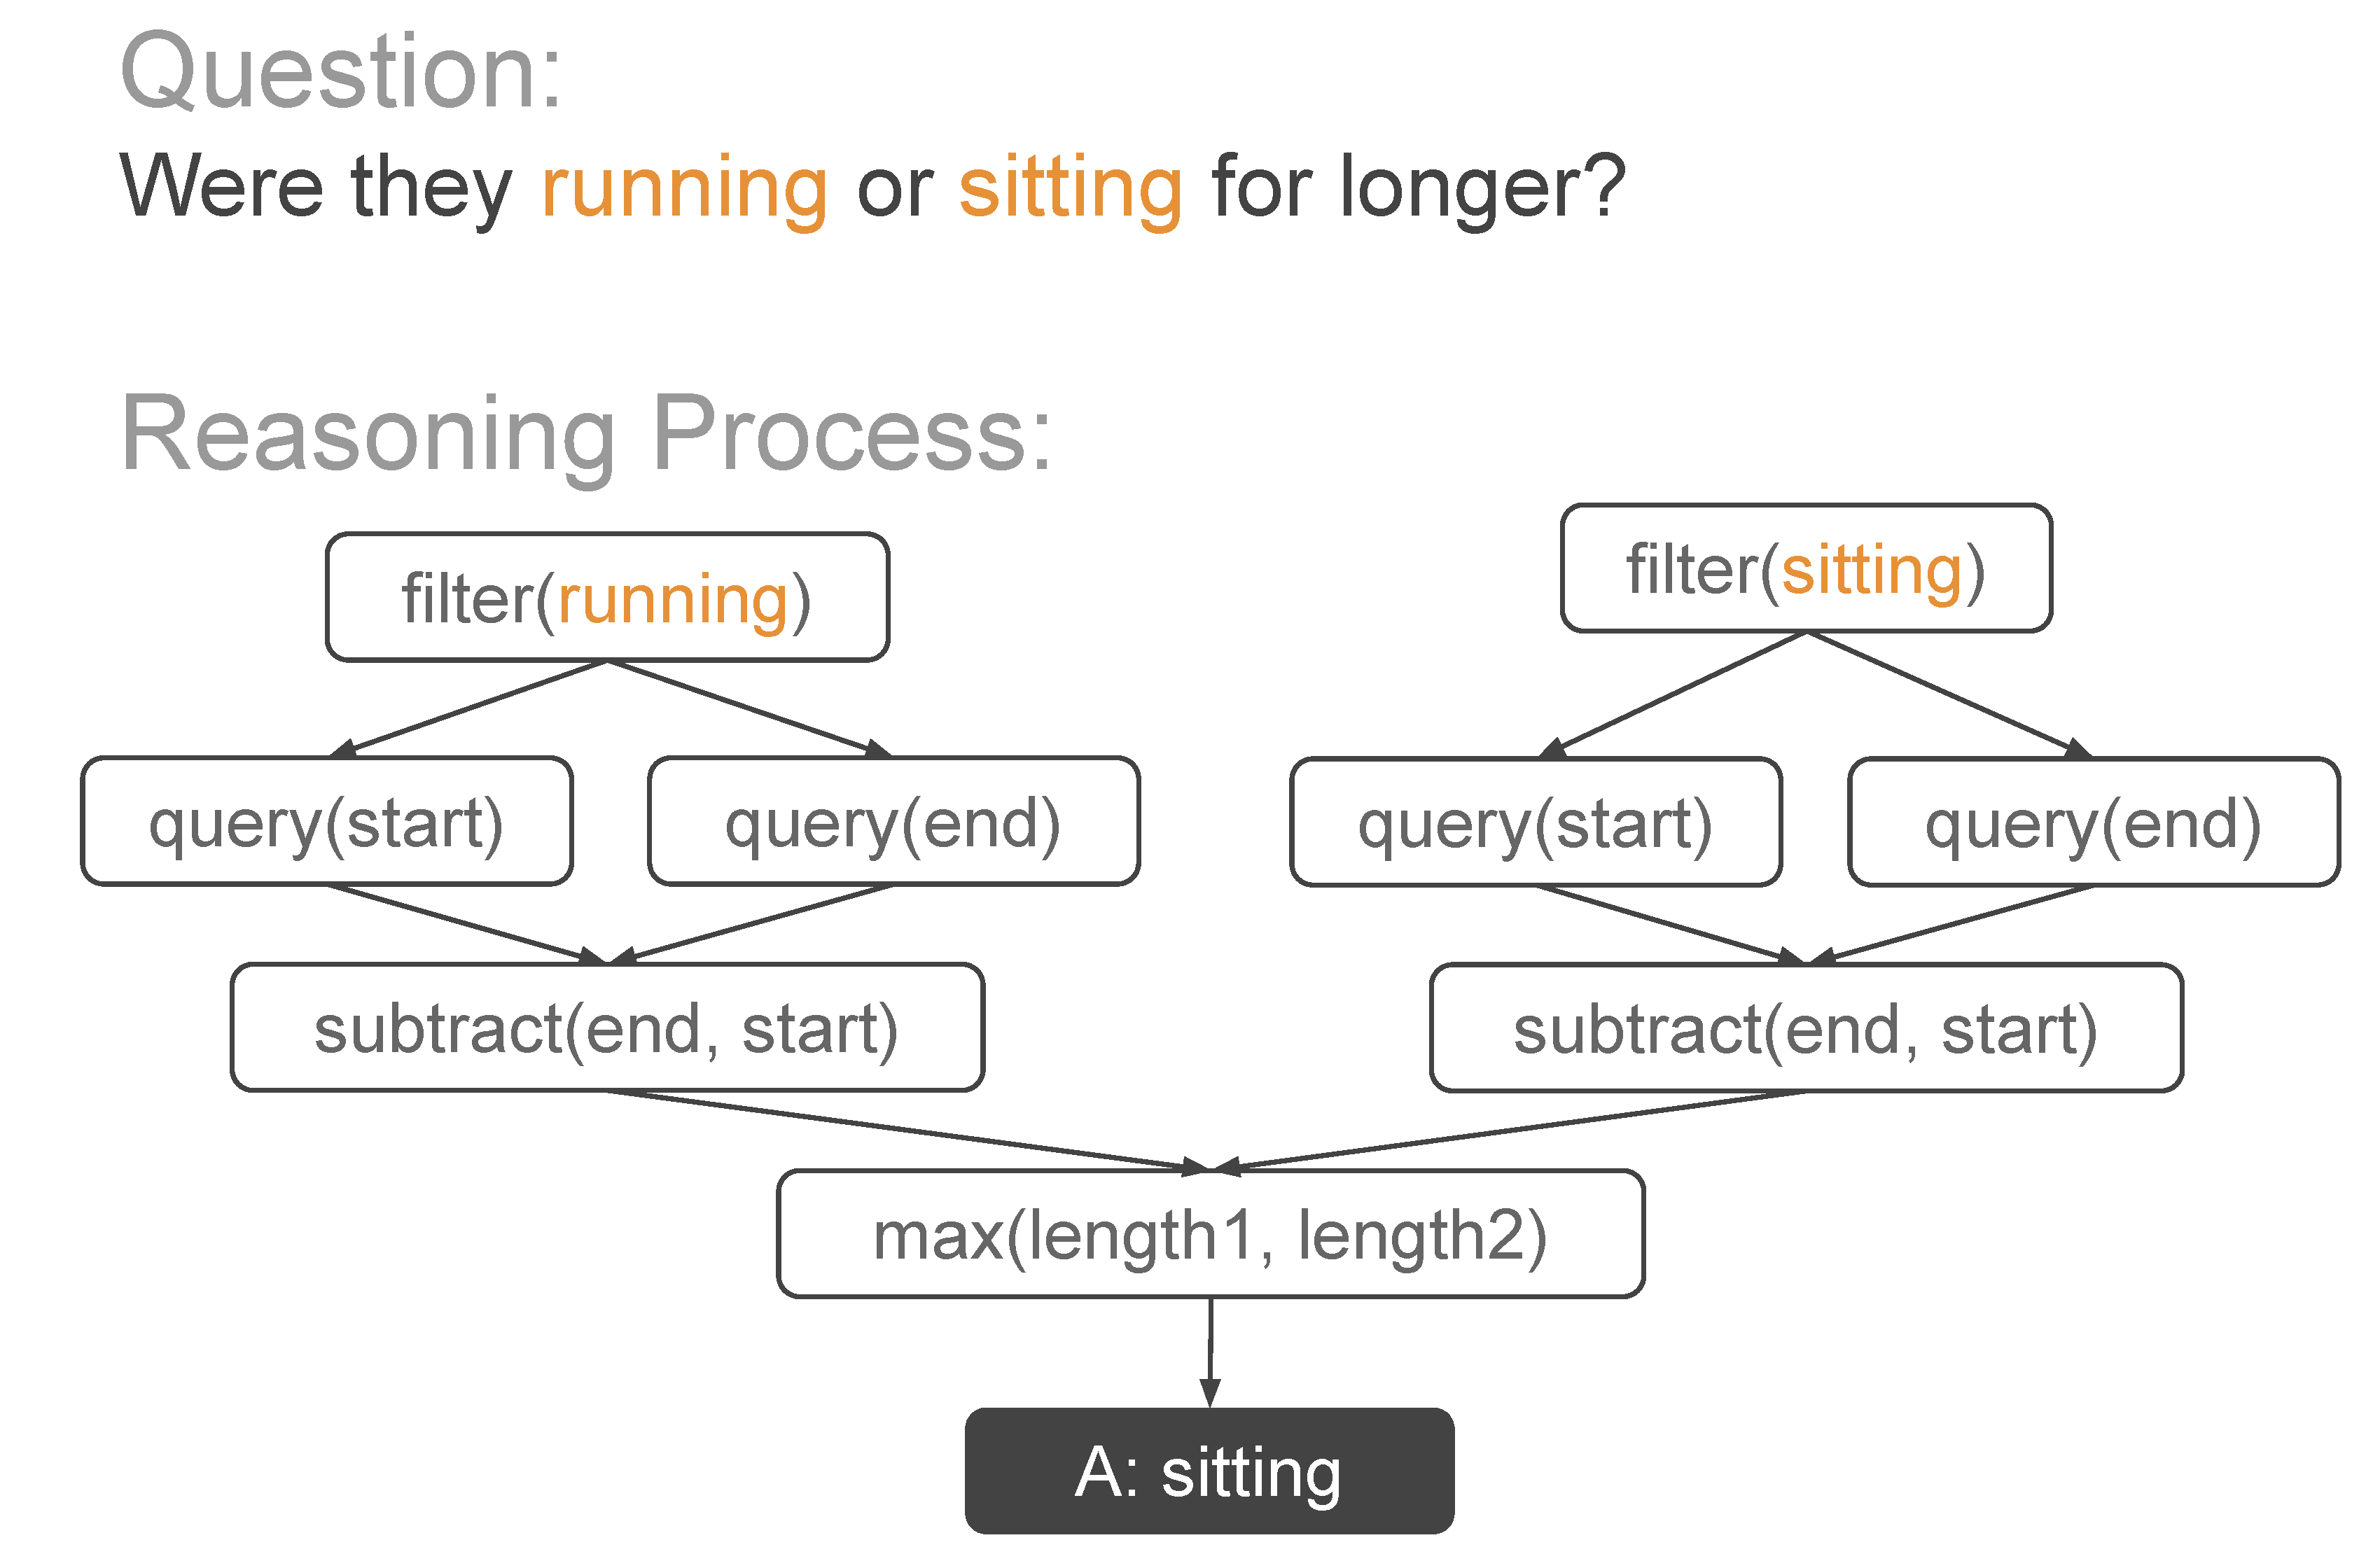
\includegraphics[width=0.95\linewidth]{figures/reasoning tree.pdf}
    \caption{TODO}
    \label{fig:tree}
\end{figure}

\begin{table*}[t]
\caption{A comparison of our AGQA with existing video question answering datasets. AGQA is orders of magnitude larger than all existing question answering datasets. It is also the first
large-scale real-world video question answering database providing both action, object, and relationship grounding.}
\label{tab:dataset_compare}
\resizebox{\linewidth}{!}{%
\begin{tabular}{@{\extracolsep{4pt}}l lrc ccccl ccc@{}}
 \multirow{2}{*}{Dataset} & \multicolumn{3}{c}{Video} & \multicolumn{4}{c}{Question answers} & \multicolumn{3}{c}{Grounding} \\ 
 \cline{2-4}\cline{5-8}\cline{9-11}
 & Avg. Length (s) & \# Videos (K) & Real-world & Not Dialogue Related & Open Answer & Compositional & \# QA Pairs & objects & relationships & actions \\ 
 \hline
MarioQA~\cite{mun2017marioqa} & 3-6 & 188 &  & \checkmark & \checkmark & & 188K \\
CLEVRER~\cite{yi2019clevrer} & 5 & 20 &  & \checkmark & \checkmark & \checkmark & 282K & \checkmark & \checkmark & \checkmark\\ \hline
Pororo-QA~\cite{kim2017deepstory} & 1.4 & 16.1 & \checkmark &  &  & & 9K \\
MovieQA~\cite{tapaswi2016movieqa}  & 202.7 & 6.77 & \checkmark &  &  & & 6.4K \\
SocialIQ~\cite{zadeh2019social} & 99 & 1.25 & \checkmark &  &  & & 7.5K \\
TVQA~\cite{lei2018tvqa} & 76.2 & 21.8 & \checkmark &  &  & \checkmark & 152.5K \\
MovieFIB\cite{maharaj2017dataset} & 4.9 & 118.5 & \checkmark & \checkmark & \checkmark & & 349K \\
TGIF-QA~\cite{jang2017tgif} & 3.1 & 71.7 & \checkmark & \checkmark & \checkmark & & 165.2K \\
MSVD-QA~\cite{xu2017video} & $<$10 & 1.97 & \checkmark & \checkmark & \checkmark & & 50.5K \\
Video-QA~\cite{zeng2016leveraging} & 45 & 18.1 & \checkmark & \checkmark & \checkmark & & 175K \\
MSRVTT-QA~\cite{xu2017video} & 10-30 & 10 & \checkmark & \checkmark & \checkmark & & 243K \\
ActivityNet-QA~\cite{yu2019activitynet} & 180 & 5.8 & \checkmark & \checkmark & \checkmark & & 58K \\
\hline
\textbf{AGQA} & 30 & 9.6 & \checkmark & \checkmark & \checkmark & \checkmark &  \textbf{1.7M} & \checkmark & \checkmark & \checkmark\\
\end{tabular}}
\end{table*}


\section{Related Work}
Our work lies within the field of video understanding using language, specifically targetted towards the visual question answering task. We use spatio-temporal scene graphs to generate our questions, and provide a suite of new evaluation metrics to measure compositional reasoning.

%\noindent\textbf{Video understanding} Video understanding encompasses a large variety of tasks including action recognition \cite{fernando2016discriminative,song2016multimodal}, action localization~\cite{anne2017localizing,gao2017tall}, and future action prediction~\cite{nagarajan2020ego}, captioning~\cite{gan2017semantic,guadarrama2013youtube2text,venugopalan2015sequence,krishna2017dense}, commonsense understanding~\cite{park2020visualcomet}, and predicting social dynamics in movies~\cite{vicol2018moviegraphs}.  While all of these tasks require some form of compositional spatio-temporal comprehension, they do not explicitly measure anything beyond test set accuracy. Our work provides an explicit benchmark with metrics that explicitly measure generalization to longer videos, novel compositions, and indirect references to objects.

\noindent\textbf{Image Question answering benchmarks.}
A wide variety of visual question answering benchmarks have been created over the past five years~\cite{johnson2017clevr,hudson2019gqa,antol2015vqa,zellers2019recognition,goyal2017making,krishna2017visual,zhu2016visual7w,kim2020answering}. These benchmarks vary in input, from synthetic datasets~\cite{johnson2017clevr}, to cartoons~\cite{antol2015vqa}, to charts~\cite{kim2017deepstory}, to real-world images~\cite{hudson2019gqa,krishna2017visual,zhu2016visual7w,goyal2017making,zellers2019recognition,antol2015vqa}. They also vary in the type of questions asked, including descriptive (who, what, where, when, which, why, how)~\cite{zhu2016visual7w}, commonsense reasoning~\cite{zellers2019recognition}, spatial compositional reasoning~\cite{johnson2017clevr,hudson2019gqa}, and spatial localization~\cite{zhu2016visual7w,krishna2017visual,hudson2019gqa}. These benchmarks facilitated the development of many models architectures and learning algorithms explicit demonstrate spatial compositional reasoning abilities~\cite{lu2016hierarchical,vatashsky2020vqa,chen2020counterfactual}. However, none of these measure temporal reasoning beyond guessing common sense actions that usually require external knowledge~\cite{zellers2019recognition}. We are inspired from the work in spatial compositional reasoning and generalize to spatio-temporal compositional reasoning in videos.

\noindent\textbf{Video Question answering benchmarks.}
As we display in Table~\ref{tab:dataset_compare}, there is a growing interest in measuring the video reasoning capabilities using question answering~\cite{tapaswi2016movieqa,lei2018tvqa,jang2017tgif,kim2017deepstory,xu2017video,maharaj2017dataset,zeng2016leveraging,yu2019activitynet,yi2019clevrer}. Unfortunately, several of these prominent benchmarks rely on dialogue and plot summaries instead of reasoning over only the visual contents~\cite{lei2018tvqa,tapaswi2016movieqa,kim2017deepstory,zadeh2019social}, resulting in models with a stronger dependence on the dialogue input than on the visual input, reducing their effectiveness at measuring visual spatio-temporal reasoning~\cite{tapaswi2016movieqa,lei2018tvqa}.

Some video-only question-answering benchmarks are synthetically generated~\cite{yi2019clevrer, mun2017marioqa}, which affords the granular control necessary to measure model abilities like causality~\cite{yi2019clevrer}, or counting~\cite{mun2017marioqa}. However, they use short video clips, utilize only a handful of objects and lack the visual diversity of real-world videos. Furthermore, they do not focus on human object interaction and activities as we do. Other video-only question answering benchmarks suffer from biases and simplicity associated with human generated questions~\cite{yu2019activitynet,tapaswi2016movieqa,jang2017tgif,lei2018tvqa} or descriptions~\cite{xu2017video,zeng2016leveraging}. The largest human-annotated~\cite{lei2018tvqa} and generated~\cite{maharaj2017dataset} datasets contain $152.5K$ and $349K$ questions and refer to videos of less than $10$ seconds long. In comparison, our corpus is purely vision based, works on videos of $2-194$ seconds long, and evaluates complex and multi-step temporal reasoning.



% Many questions relevant to reasoning over videos require multi-step reasoning. A simple example covered by current datasets involves first localizing in time, then reasoning about that specific time. For example, this question from~\cite{jang2017tgif}, "What does the model do after lower coat?", requires finding when the model lowers her coat, then determining her activity after that. Another way to reason compositionally \mgm{is this a word?} is to refer to subjects indirectly, as the ImageQA benchmark~\cite{hudson2019gqa} does with "What color is the food on the red object to the left of the girl?". We use both temporal localization and indirect references to increase question compositionality, and we implement several metrics to measure different compositional reasoning abilities than existing Visual Question Answering benchmarks.

%Existing question-answering benchmarks are limited in the diversity of their questions. Since most benchmarks are image-based, they only test a model's reasoning over spatial relationships~\cite{johnson2017clevr,hudson2019gqa,antol2015vqa,goyal2017making,krishna2017visual,zhu2016visual7w}, object attributes~\cite{johnson2017clevr,hudson2019gqa, antol2015vqa,goyal2017making,krishna2017visual}, and common sense understanding~\cite{zellers2019recognition,antol2015vqa,krishna2017visual}. These benchmarks are unable to test reasoning over temporal relationships or activities beyond guessing based on common sense knowledge \cite{zellers2019recognition}. All questions asked by VideoQA benchmarks on non-synthetic videos that do not include extra textual information like dialogue limited temporal localization. Temporal localization refers to using the phrase "before/after/while $<$action$>$" to localize a relevant time in the video over which to reason. Questions in these benchmarks 1) can be answered from a single frame of the video, 2) apply to the entire video with no temporal localization, or 3) ask "what happened before/after/while $<$action$>$?"~\cite{jang2017tgif,xu2017video, maharaj2017dataset, zeng2016leveraging, yu2019activitynet}. Of the questions that apply to the entire video, some spatio-temporal topics are measured like counting and object and action recognition.


\noindent\textbf{Scene graphs.}
Scene graphs were first introduced as a Cognitive Science~\cite{biederman1982scene,wolfe1998visual} inspired representation for static images~\cite{krishna2017visual}. Each scene graph encodes objects as nodes in the image and pairwise relationships between objects as directed edges connecting nodes. 
%For example, an image with a \object{person} \relationship{throwing} \object{frisbee} would represent \object{person} and \object{frisbee} as nodes with a directed edge between them to represent \relationship{throwing}. 
The Computer Vision community has utilized the scene graph representation for a variety of tasks including visual question answering~\cite{johnson2017inferring}, relationship modeling~\cite{lu2016visual}, object localization~\cite{krishna2018referring}, evaluation~\cite{anderson2016spice}, generation~\cite{johnson2018image,ashual2019specifying}, retrieval~\cite{ashual2019specifying,johnson2015image}. Of particular interest to our project is how scene graphs from Visual Genome~\cite{krishna2017visual} were used by create GQA, a benchmark for compositional spatial reasoning over an image~\cite{hudson2019gqa}. Our work is a generalization of GQA's pipeline --- our pipeline develops templates that reason over not just objects and their relationships but also over how those relationships change over time to form different actions. We develop templates and programs that operate over Action Genome's recently released spatio-temporal scene graphs~\cite{ji2020action}.

\noindent\textbf{Compositional reasoning.}
While there are numerous definitions of compositionality, we in particular use what is more colloquially referred to as bottom-up compositionality --- ``the meaning of the whole is a function of the meanings of its parts''~\cite{cresswell1973logics}. In our case, reasoning about the question ``Was the person running or sitting for longer?'' requires finding the start and end of when the person was running and sitting, subtracting the start from the end, then comparing the lengths (Figure~\ref{fig:compo_fig}). Unfortunately, the most popular benchmarks and metrics defined to study compositional behavior have been limited to synthetic environments~\cite{keysers2019measuring,lake2018generalization,johnson2017clevr,yi2019clevrer} or to static images~\cite{hudson2019gqa}. Recent work has argued the importance of compositionality in enabling models to generalize to new domains, categories, and logical rules~\cite{lake2018generalization,vatashsky2020vqa} and have discovered that current models struggle with multi-step reasoning~\cite{fan2019heterogeneous}. These studies motivate a benchmark like ours that define multiple metrics to explore compositional reasoning in real-world videos.




\begin{figure*}[t]
    \centering
    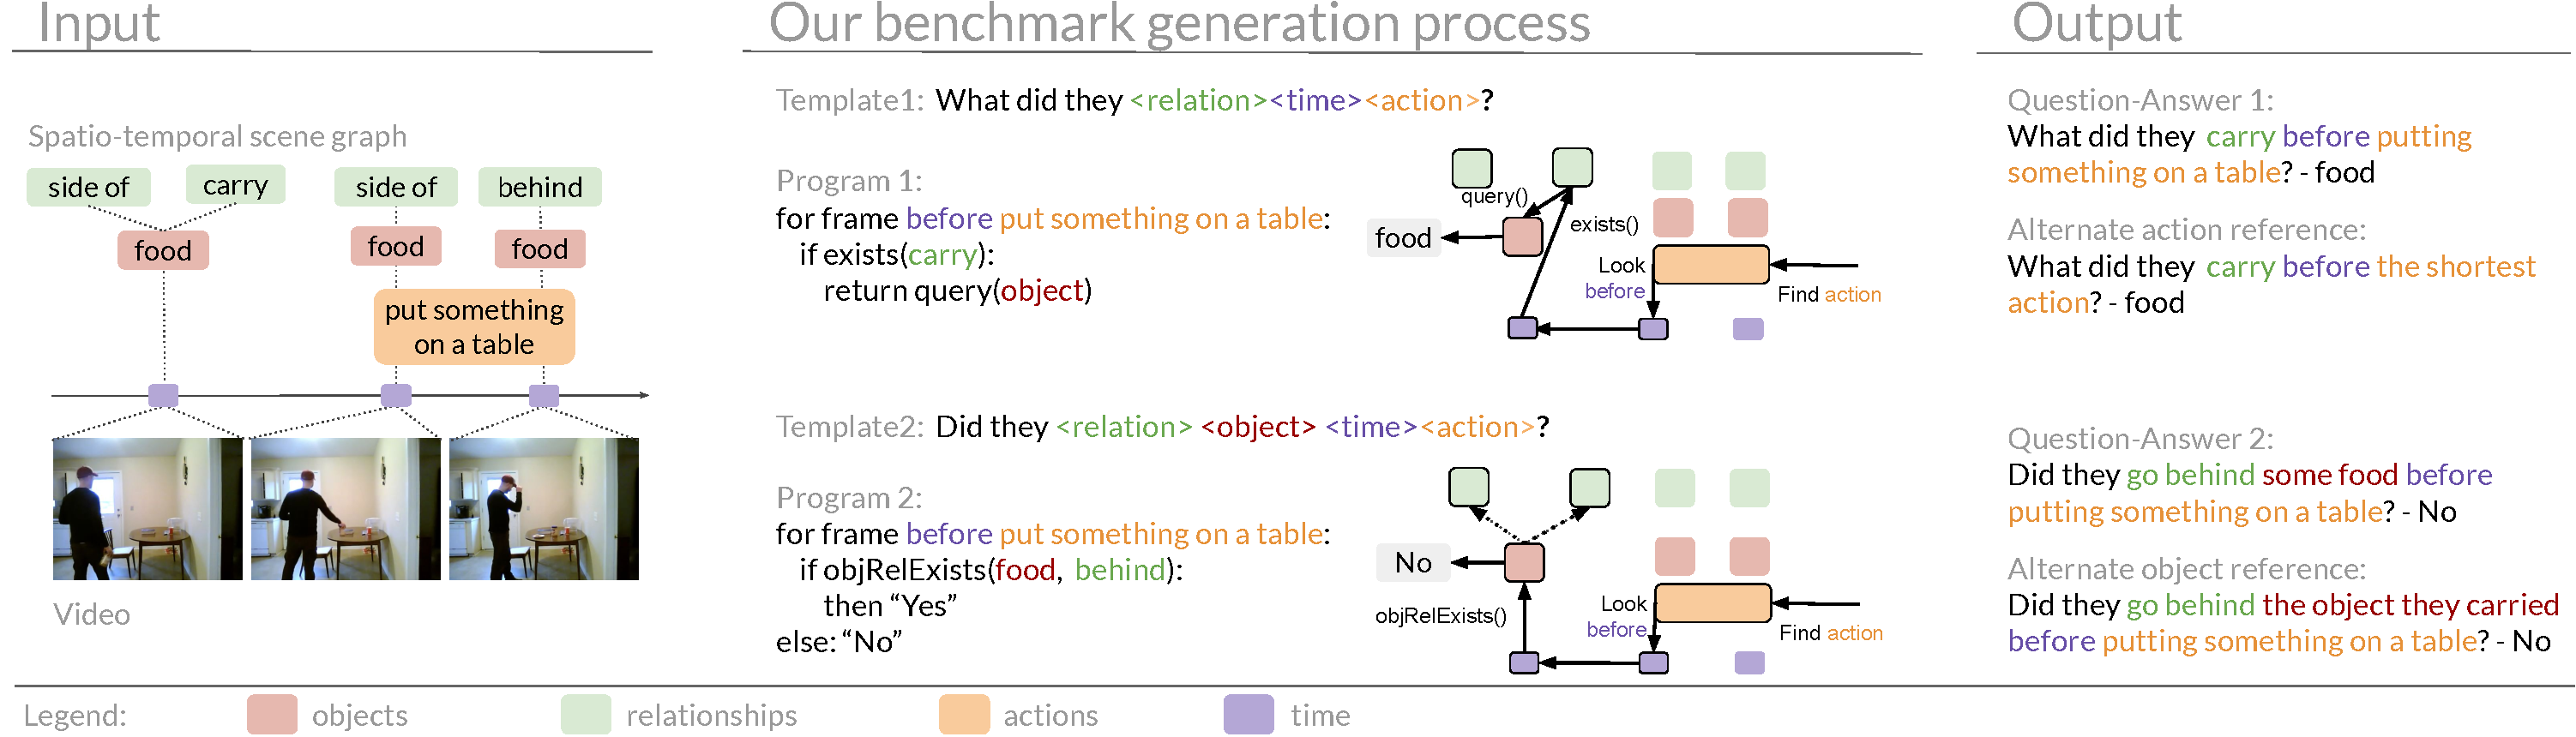
\includegraphics[width=0.95\linewidth]{figures/system.pdf}
    \caption{\textbf{Input:} To generate questions, we first ground the video in the \object{object}, \relationship{relation}, \action{action}, and \temporal{frame} level visual primitives by augmenting Action Genome's spatio-temporal scene graphs~\cite{ji2020action} and Charades' action annotations~\cite{sigurdsson2016hollywood}. \textbf{Our benchmark generation process:} we built a series templates with $<$tags$>$ that can be filled in with the associated primitive to generate a natural language question. Each template is also associated with a unique program that reasons over the spatio-temporal scene graph to automatically generate the answer to the question. \textbf{Output: } We create a dataset of question-answer pairs. Question diversity is increased by referencing primitives by their qualities (e.g. 'shortest action') or interactions (e.g. 'the object they carried').}
    \label{fig:system}
\end{figure*}

\section{Dataset Generation}

Inspired by GQA's pipeline, we generate questions by combining the content of scene graph annotations with question templates~\cite{hudson2019gqa}. Unlike GQA, we use spatio-temporal scene graphs and create new question templates that include a wider variety of temporal reasoning concepts. 

\subsection{Spatio-temporal Scene graphs}

The spatio-temporal scene graphs from Action Genome annotate videos from the Charades dataset about the relationships between a subject and objects over time \cite{ji2020action, sigurdsson2016hollywood}. These videos range in length from 2-194 seconds and are filmed by Amazon Mechanical Turk workers performing skits in their own homes.

\mgm{Delete from this paragraph as space requires - and move to supplementary}
We augment Action Genome's spatio-temporal scene graphs to make the content better suited for quality questions. First, we combined the spatio-temporal scene graph annotations with the Charades action annotations to create a new scene graph with action nodes and denser object and relationship annotations. Next, since the exact second that actions begin and end is often unclear for humans, we add in prior knowledge about actions and adjust the annotations accordingly. For example, it can be assumed that if someone is annotated as "holding a cup" and "putting a cup somewhere" at the same time, they hold the cup first before putting it somewhere. We add in relationship entailments, so that if someone is annotated as "carrying" an object, they are also annotated as "holding" and "touching" it. We took out the attention relationship "looking at" and the negative relationships "not looking at" and "not contacting", and unclear relationships like "unsure" and "other relationship" because those create questions that are difficult for humans to answers. We also simplify the number of objects and actions referred to in a single video, getting rid of references to the same item in the video by multiple phrases. With these and other adjustments, the spatio-temporal scene graphs became densely annotated and referred to objects and events in the video more consistently. This series of edits addressed some of the annotation errors or priors in Action Genome and Charades that lead to non-sensical or incorrect answers. However, some errors in annotations persist and do carry over into our questions. [AMT results preview here?]

After making these corrections, our spatio-temporal scene graphs have 28 objects, 54 relationships, and 157 actions. There are 7,787 training set and 1814 test set scene graphs that fill in question templates.

\subsection{Question Templates}

The second part of the pipeline consists of question templates that each have natural language sentences with tags representing different elements categories in the video, such as in the question "What were they $<$contact relationship$>$?". These tags can be objects, relationships, actions, or phrases that reference a certain part of the video. To increase variety in the dataset, there are multiple natural languages options for each template and the input objects, relationships, and actions are adjusted to be grammatically correct.

\mgm{Moved form experiments section, since we want to talk about diversity in reasoning here}
\textbf{What: } These questions ask what a person was doing. They measure the ability to locate a relationship and determine what object is being used. \mgm{this expl will change if we add in actions}

\textbf{Length: } The length category compares the length of different actions. When generating the questions, we add in a buffer so an action must be annotated as at least 7 seconds longer than another for them to be compared. Length questions are only binary because they are comparisons (e.g. "What did they do for longer $<$action1$>$ or $<$action2$>$) or verification questions (e.g. "Did they do $<$action1$>$ for less time than $<$action2$>$.

\textbf{First and Last: } These questions about the first or last occurrence in the video. 


\textbf{Sequencing: } These questions ask if an action comes before or after another action.

\textbf{Count: } Count questions ask how many times an action occurred, or ask to compare the number of times two actions occur.

\textbf{Exists: } These questions ask if some event occurred



Each template also contains information about the question's structure and the objects, relationships, and actions it references. Finally, each template contains a program that reasons over the spatio-temporal scene graph to automatically generate the answer.

Before adding the question to the dataset, we check that there is no ambiguity in possible answers. We also avoid questions that have common sense combinations ("Are they wearing clothes?"), those that give away the answer ("What did they old while holding a blanket?), and those that are nonsensical ("Were they eating a mirror?").

To generate a question-answer pair, our system combines a spatio-temporal scene graph with these templates by replacing the tags with elements of the corresponding types. For a video where the person is holding a blanket while sitting on a chair, our pipeline would create both questions "What were they holding?" and "What were they sitting on?". Given the scene graph information, we then automatically determine the answers "blanket" and "chair" respectively. We have 27 templates and 251 natural language questions with an answer space of 208. From just these 27 questions, we generate over 133 million question-answer pairs before balancing, with over 90 million unique natural language questions.

\begin{figure}[t]
    \centering
    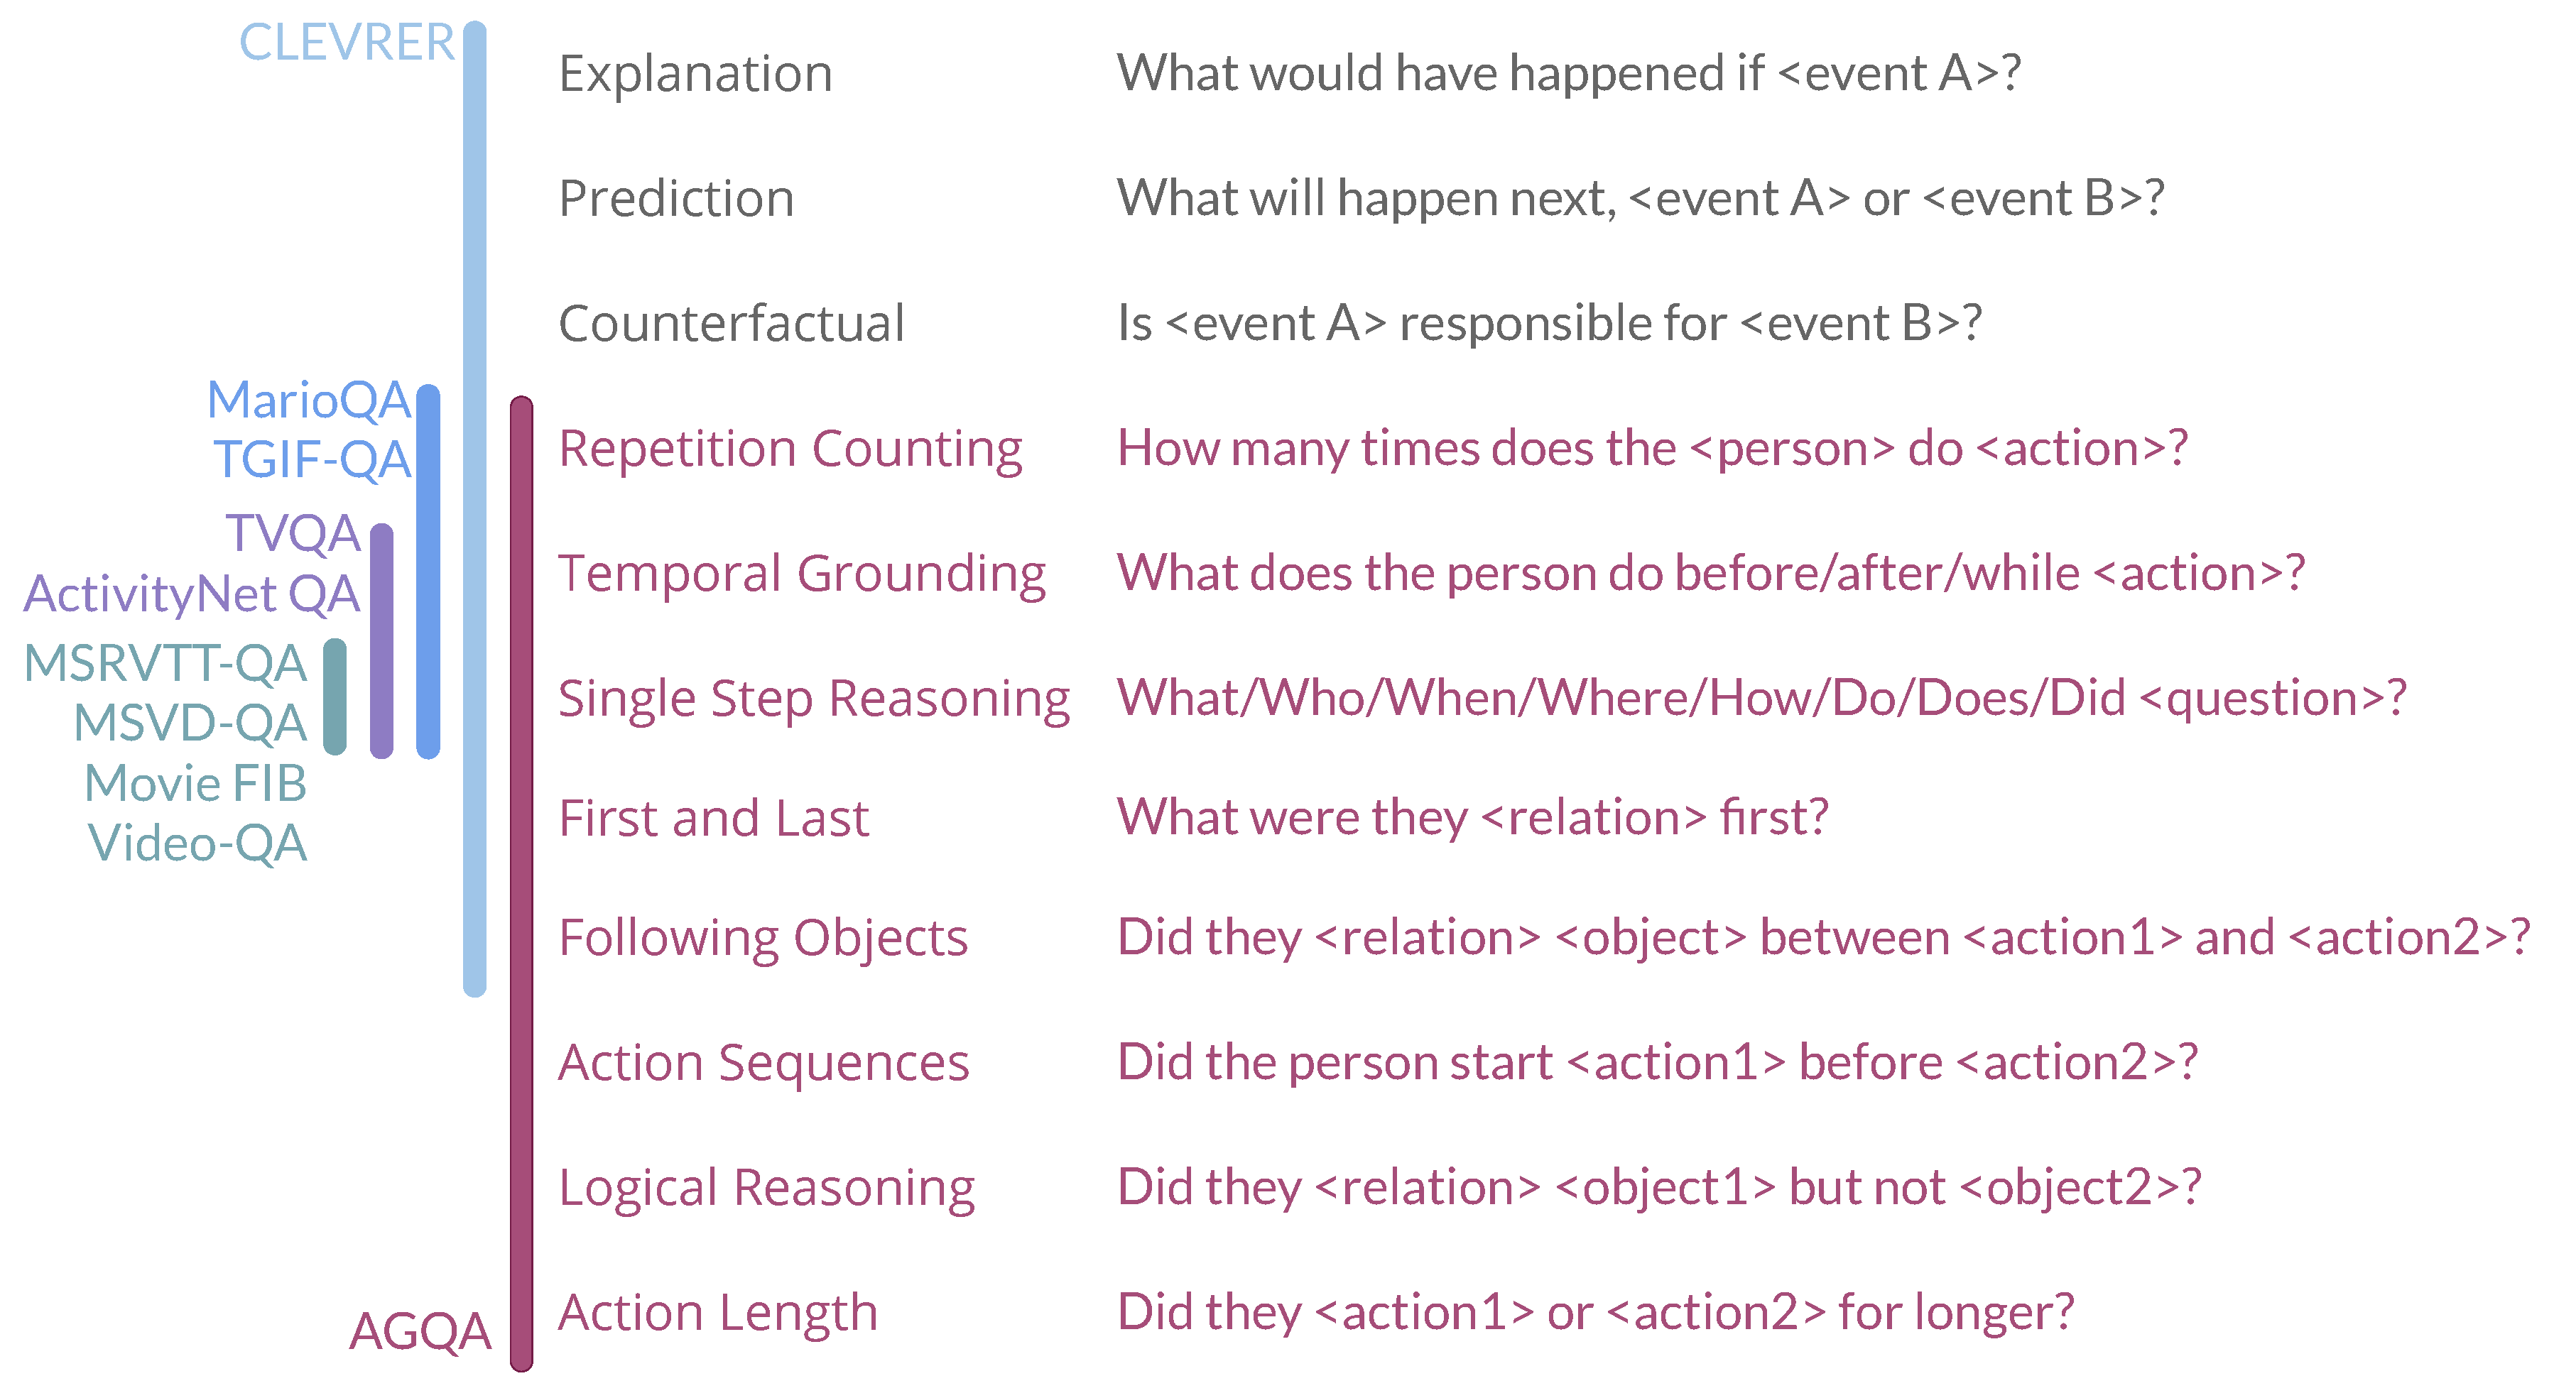
\includegraphics[width=\columnwidth]{figures/questions.pdf}
    \caption{A VideoQA benchmark should be diverse in the spatio-temporal reasoning skills it requires. Since our videos are based on skits, we do not have questions on explanation, prediction, or counterfactual reasoning as does the synthetic dataset CLEVRER~\cite{yi2019clevrer}. However, our questions cover a wider variety of reasoning abilities than other non-synthetic VideoQA benchmarks.}
    \label{fig:questions}
\end{figure}

\subsection{Creating Compositional Reasoning}

Compositional reasoning in questions means that the questions require multiple steps of reasoning to answer. For example, the question "Were they opening a closet or a refrigerator before holding a bag?" requires 1) finding the time at which they hold a bag, 2) shifting attention to before that action, 3) locating when they opened something and 4) determining what object they opened. To generate complex, compositional questions, and to inform a suite of metrics looking specifically at compositional reasoning, we increase compositionality in generated questions in three ways.

First, the question templates themselves can have compositional reasoning. For example, the template "Were they $<$relation$>$ $<$object1$>$ but not $<$object2$>$?" has three reasoning steps 1) searching for if the relation-object1 pair exists, 2) searching for if the relation-object2 pair exists, and 3) a logical operator. 

Second, almost all templates have an optional $<$time$>$ tag that can be filled with a phrase "before/after/while/between $<$action$>$". When this $<$time$>$ tag is filled, the program generating the answer first looks at the indicated frames before figuring out the answer. Therefore, adding in temporal localization phrases adds compositional reasoning steps by first requiring focusing attention on a certain part of the video before continuing with the rest of the template.

Third, $<$object$>$, $<$action$>$, and $<$relation$>$ tags can be filled with both direct and indirect references. An $<$object$>$ could be referred to directly as a "blanket" or indirectly as "the object they threw". An $<$action$>$ can be referred to directly as "eating something" or indirectly as "the longest action". A $<$relation$>$ could be referred to directly as "watching" or indirectly as "the thing they did to the laptop". Since most objects have multiple relations, indirect relationships are less common. Indirect references must be figured out first before answering the rest of the question, so they increase the number of compositional reasoning steps.

Finally, these indirect references and temporal localizations can be combined to create more granular references and even more compositional reasoning steps. Combining a temporal localization with an action indirect reference gets phrases like "before the longest action". When there is ambiguity in an indirect object phrases, such as if they threw multiple things over the course of the video, increased specificity in the indirect references increases complexity (e.g. "the object they threw before going from standing to sitting" or "the object they threw first").

Several other Visual Question Answering benchmarks use compositional reasoning. Our method for creating compositionality is most similar to GQA. However, while GQA uses attributes (e.g. "red") and spatial relations (e.g. "to the left of") as object indirect references, we have temporal localizations, action indirect references, and object indirect references focused on their relationship with the subject \cite{hudson2019gqa}. 

CLEVRER is the VideoQA dataset that thus far most explicitly incorporates compositional reasoning. However, their subjects are somewhat different. They add in compositionality with descriptions of objects (shape, color, material), motion, collision, and temporal ordering. We refer to objects by their interaction with the subject, look at real life videos, and use indirect references in conjunction with other spatio-temporal reasoning skill \cite{yi2019clevrer}.

Of other real-world video question answering sets, TVQA has a similar temporal localization process, but they do not refer to other subjects indirectly, and their questions rely on dialogue and don't have as many reasoning steps built into the template \cite{lei2018tvqa}. All other benchmarks that use temporal localization only ask "What did they do $<$temporal localization$>$?", whereas ours adds in temporal localizations to already complex templates. Finally these real-world VideoQA benchmarks do not systematically add in compositional reasoning in a way that allows it to be specifically measured in metrics. 



\begin{figure}[t]
    \centering
    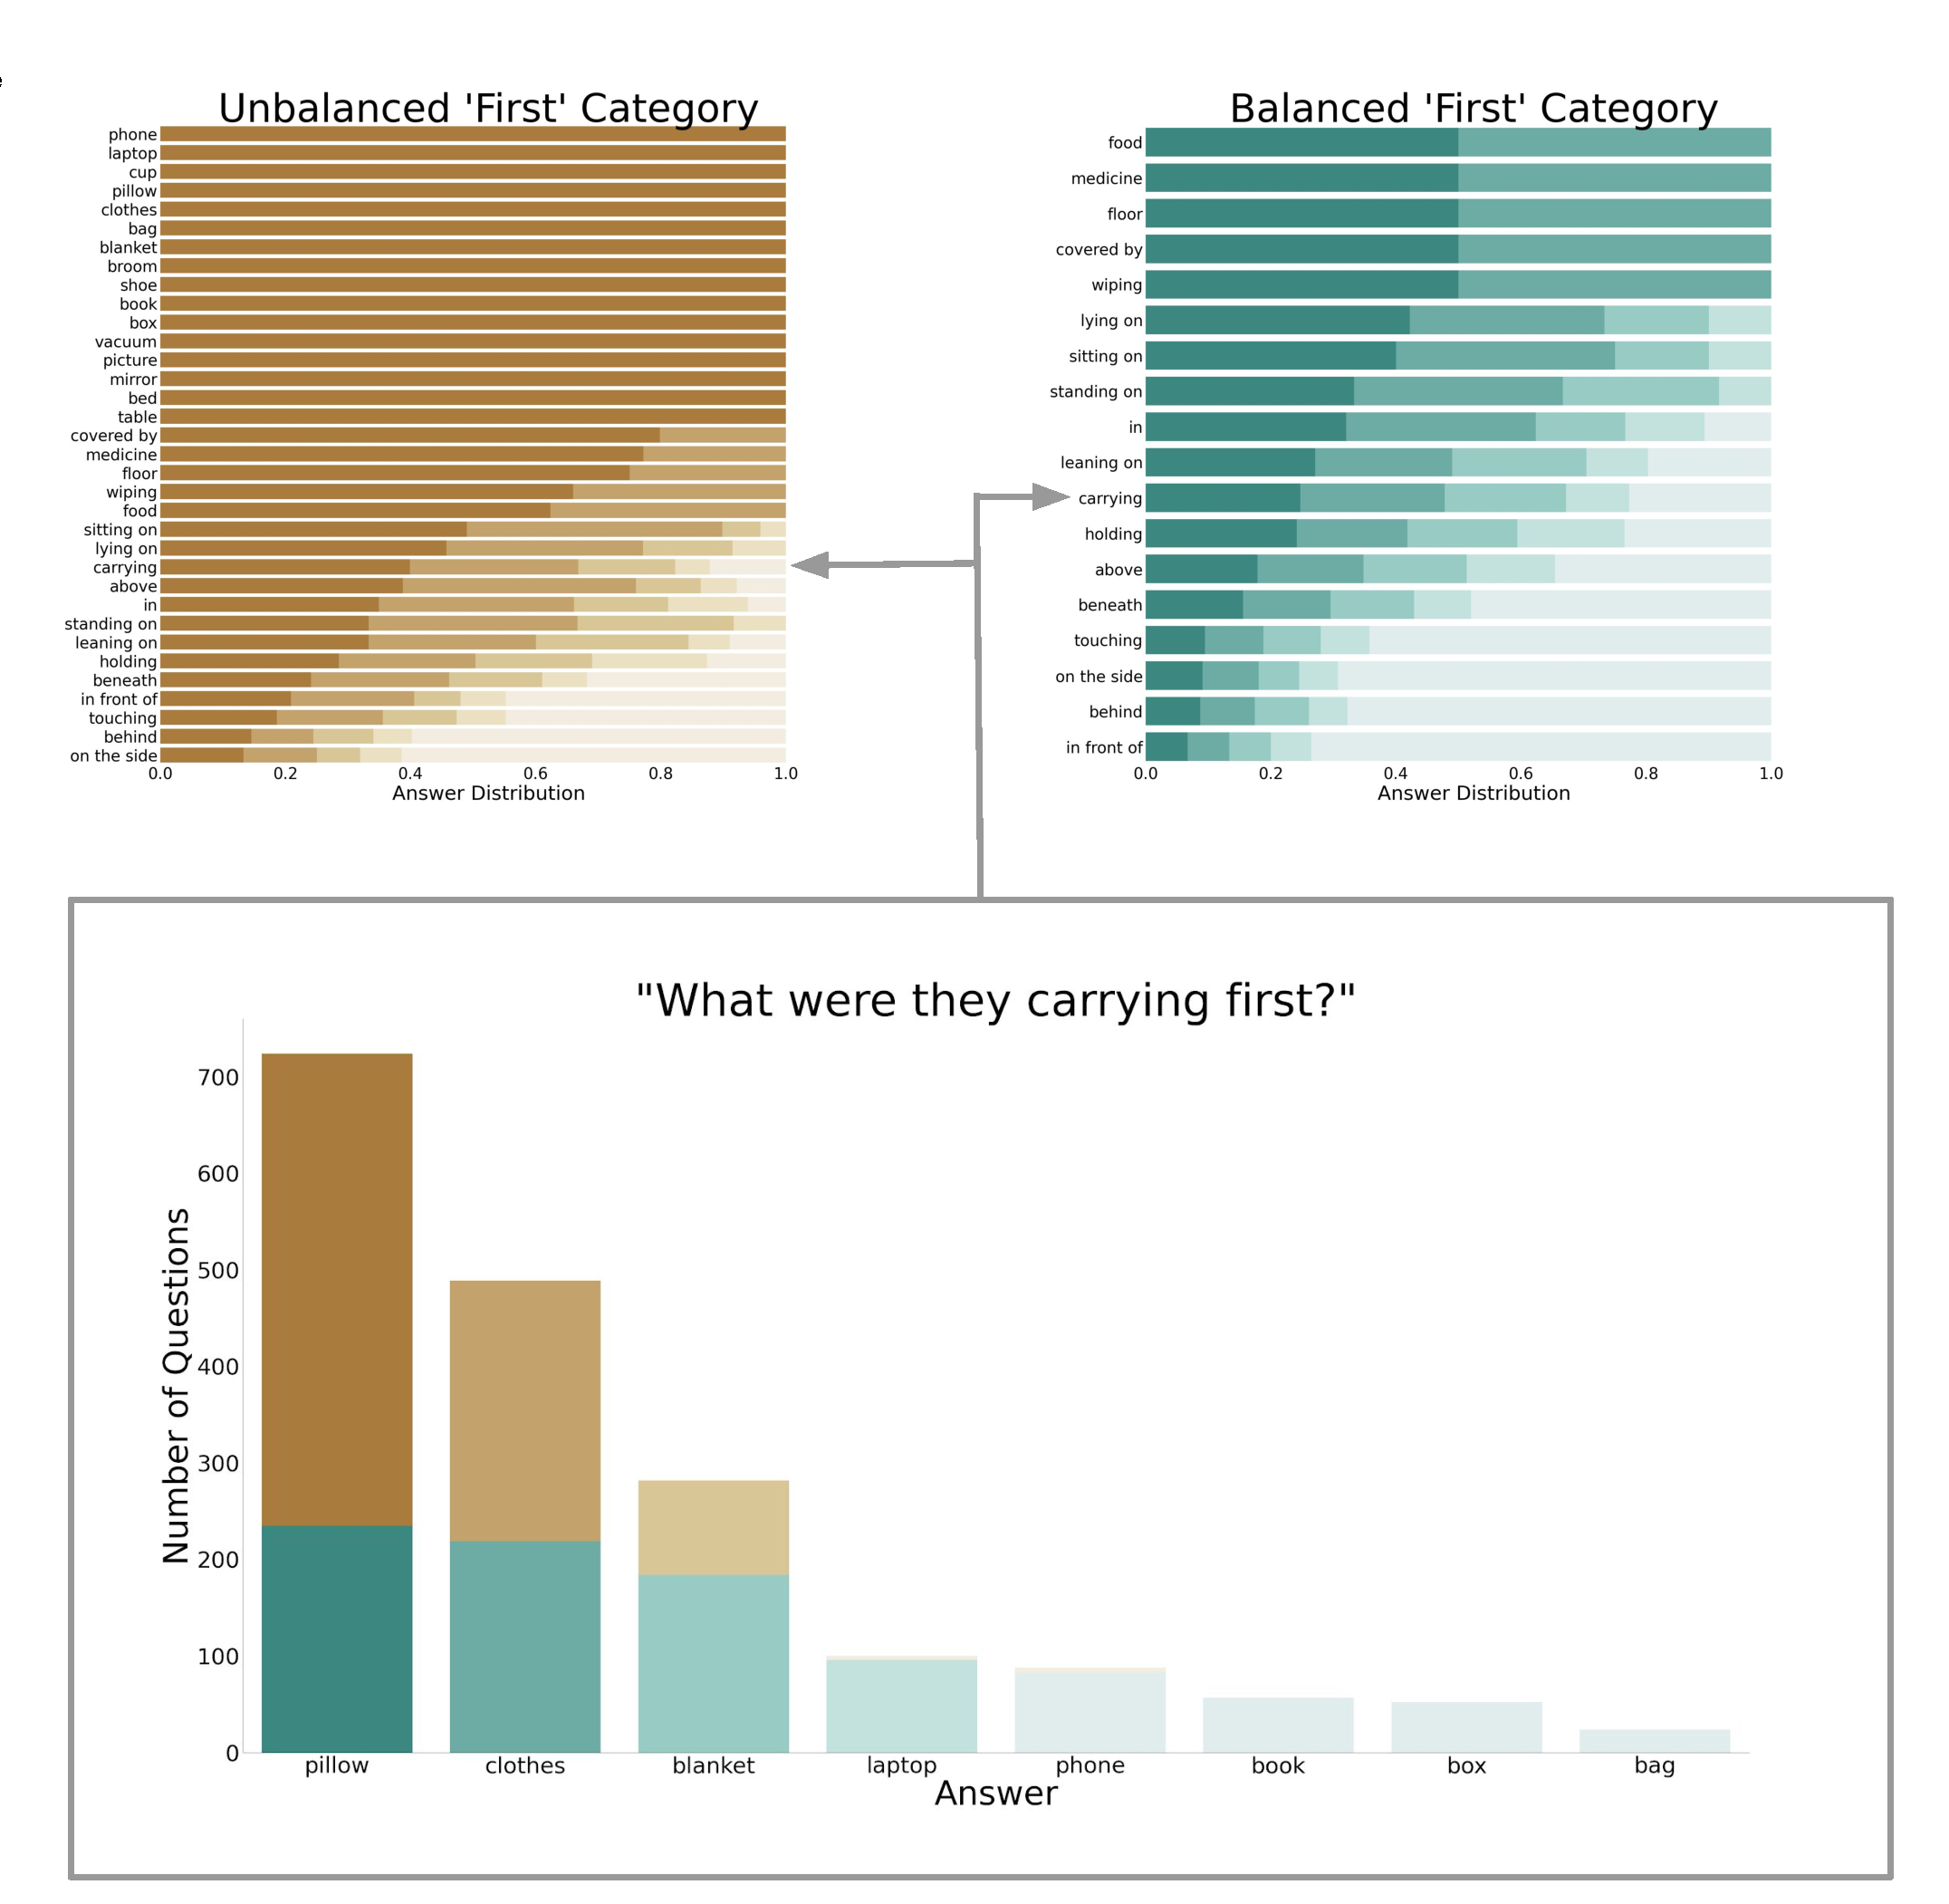
\includegraphics[width=0.95\linewidth]{figures/balance first.pdf}
    \caption{To avoid an artificially easy task, questions should have a diverse set of answers. The bottom row shows the answer distribution for questions that ask "What were they carrying first". In the unbalanced set, the answer "pillow" is correct for nearly 40\% of questions, while after balancing that value drops to 25\%. This balancing effect occurs across all question categories, as seen in the top row.}
    \label{fig:balancefirst}
\end{figure}


\subsection{Balancing}

Machine Learning models are notoriously good at taking advantage of imbalances in the dataset to improve accuracy scores without using the reasoning skills we want to evaluate \cite{hudson2019gqa, goyal2017making, johnson2017clevr, mariani2018bagan, shorten2019survey}. Domains like object detection and image classification have addressed unbalanced datasets by manipulating the image in various ways or using GANs to make categories more balanced \cite{mariani2018bagan, shorten2019survey}. Many VQA datasets contained real world priors exacerbated by human annotation bias, resulting in inflated accuracy scores and a lack of understanding of the actual reasoning abilities of these models~\cite{goyal2017making,hudson2019gqa}. However, balancing answer distributions for the VQA task is difficult for human generated datasets because low control over the content of each question, since often priors in the types of answers each question gets, and because manipulating a natural image in a way that changes the answer of a question is a more difficult task than rotating an image. Previous work reduced imbalances in VQA datasets by reducing skews in the answer distribution \cite{hudson2019gqa, goyal2017making, johnson2017clevr}.

 %For example, in the VQA1.0 dataset, 41\% of answers for questions starting with "What sport is..." were "Tennis". These types of priors meant that models could answer over 50\% of the questions correctly without considering the visual input~\cite{goyal2017making}. Once these issues came to light, some new benchmarks attempted to mitigate these biases. VQA2.0 took many of the questions from VQA1.0 and added a similar picture leading to a different answer. This procedure helped, but was only applied to 71\% of questions due to annotation difficulties. Blind models measured on VQA2.0 could still answer 67\% of binary questions and 27\% of open answer questions correctly without seeing visual input~\cite{hudson2019gqa} \mgm{our open answer blind model is similar... so this point is less salient unless we can bring that down}. 
In the ImageQA task, VQA2.0 took many of the questions from VQA1.0 and added a similar picture leading to a different answer~\cite{goyal2017making}. Synthetic datasets like CLEVR and CLEVRER are able to balance their input because they have tight control over what examples are generated \cite{johnson2017clevr, yi2019clevrer}. The GQA dataset addressed these biases by smoothing the answer distribution by question category. This balancing of the answer distribution retains but reduces the power of real world priors ~\cite{hudson2019gqa}. 

In the Video Question Answering world, CLEVRER creates the most balanced dataset, but it's synthetic generation of videos and limited questions make that an easier task than balancing answer distributions on real-world videos \cite{yi2019clevrer}. On real-world videos, \cite{yu2019activitynet} balances it's yes and no questions and ensures certain categories make up at least 10\% of the dataset. AGQA balances its answer distributions most similarly to GQA that creates smoother distributions at a more granular level than existing real-world VideoQA datasets. 

Our balancing process was adjusted from GQA's. Questions are sorted into global and local categories. Global categories discuss the overall subject of the question (e.g. "counting" or "length"), while local categories are specific to the content of the question (e.g. "counting-throwing some clothes" or "length-running"). Questions also have two answer types, binary and open. Binary questions have two possible answers, such as "Yes/No" or "Before/After". Unlike GQA, we categorize questions that present a choice between two objects, like "Were they to the side of a closet or a bed?", as binary questions as well. Open questions have open-ended answers like "What were they carrying?". 

For binary questions, each local category is balanced such that each possible answer is 50\% likely. For example, for all questions with the base idea "Did they take a blanket from somewhere or go from standing to sitting more times?', half of the questions have "take a blanket from somewhere" as an answer, and half have "go from standing to sitting" as an answer. 

For open questions, we first balanced the global category, then each individual local category. The balancing procedure first truncated 1\% of questions making up the tail of the distribution. \mgm{may want to have a separate algorithm aside to describe this idk. It's a bit of a mouthful} Then, starting with the most popular answer as the "head" it deletes answers in the "head" randomly until either the the proportion of the number of answers in the head and the tail, is less than some number b, or if deleting anymore would change the order of the answer distribution from most frequent to least frequent. Then, the head is expanded to contain an extra answer, and the process repeats. This entire process repeats with b decreasing at every iteration until either half the questions have been deleted, or the most common 20\% of answers made up less than 30\% of all questions. \mgm{Do we need to explain where got the numbers from? It was mostly just experimenting} \mgm{Will be turning this into a figure. }

We then balanced on the structural question types. Query questions are open ended, compare questions compare the qualities of two items, choose questions choose the correct answer from two options, logic questions use logical operators, and verify questions verify if the ideas presented in the question are correct or not. Some templates, especially those with Yes/No answers, had more tags and therefore produced more questions per video. To keep the benchmark challenging with open ended questions, we balanced such that 'query' questions with truly open answers make up half of the dataset.  \mgm{Have a table with the structure, a description, \% before balancing and \% after balancing. Figure for the distribution before and after.}

Finally, we balanced so that for every question with a temporal localization that when added does not change the answer, there is at least one identical question where it does change the answer.

\subsection{Results}
Before balancing, our dataset has over 86.6M question-answer pairs in the training set and over 46.5M question-answer pairs in the test set. After balancing, our dataset has 1.17M question-answer pairs in the training set and 600K question-answer pairs in the test set. Figures of how the distributions changed. We contribute a large, real-world dataset that does compositional reasoning and is balanced to increase difficulty. 



\section{Experiments and analysis}

%CLEVR: First described models. They then analyzed the dataset by question type (query vs compare), relationship type (spatial vs attribute), question topology (chain vs tree-structured questions). they have an interesting section on looking at "effective" question size. They say that accuracy is not necessarily related to question size itself, so they prune functions from the program until they find the smallest functional program that when put on the scene graph creates the correct answer. This is the 'effective' program length, and that is related to difficulty. Nothing comes immediately to mind about how I would do that with AGQA though. They also looked at relative vs absolute spatial reasoning. SO if you say "left of x" they see how accurate it is if you just look in left half of the image, and then they prune when spatial relationships aren't absolutely necessary. They found that much worse on ones that require relative, not absolute, spatial reasoning. This could potentially be expanded to temporal localization. Then look at novel combinations. They have a summary in discussions and future work. 

%GQA: breaks down semantic and structural categories (does not spend much time on these),then talks about data set's vocabulary size and possible answers. We are a lot weaker on this point. GQA talks about briefly baseline experiments on blind models. They they describe transfer performance, i.e. training on VQA and testing on GQA and vice versa to show theirs is harder (we don't have an equivalent though). Then, they get into describing their new metrics and have. subsection for each category. For some of them they have a formal representation, for others they don't.

% Note to self: will need to change some to logical structural.. maybe compare?

%Notes to self: I think that the stuff CLEVR did with pruning down programs to find the essential necessities is cool. I probably don't have time for that now, but worth keeping in mind. 

First, we judge the quality of our questions through a human subject study, finding that humans achieve a 97\% accuracy on our benchmark. We then tested our suite of metrics on several recent models to measure different types of spatio-temporal reasoning skills. We found that models perform close to random on most measures. Finally, we measure compositional reasoning in several ways and find that existing models struggle on generalizing to new information, but are successful at generalizing from shorter videos to longer videos.

\subsection{Human Study}

As mentioned before, annotation errors in the Charades and Action Genome datasets could lead to confusing or incorrect questions in our dataset. To measure the level of error after our augmentation strategies, we tested Amazon Mechanical Turk workers on their ability to answer the questions. We ran the study on 300 questions over 60 videos, with two Amazon Mechanical Turk workers per video. When the two workers disagreed, we got a third worker's opinion to break the tie. Since the Charades videos were filmed in AMT worker's homes there were often many objects and actions that were not within the Charades and Action Genome annotations. To clarify the objects of interest, we listed them for the workers. Workers were first given a free form text box, then given a drop down menu of possible answers to select the closest possible answer from the words within the model's vocabulary. We measure human accuracy from accuracy with the drop down menu. 

After the first round, 28 questions had disagreement between the annotators so were rerun. With the tie breakers, human accuracy is 97\%, which implies that 3\% of our questions have errors in them. In comparison, GQA gets 89.3\% on human accuracy~\cite{hudson2019gqa}, and CLEVR gets between 79\% and 97\& depending on the question category~\cite{johnson2017clevr}. 


\subsection{Describe the models we looked at briefly}

To test different subsets of the dataset, we look at three state of the art models. The Hierarchical Conditional Relation Network (HCRN) consists of... 


\mgm{Is it necessary to do this? CLEVR did, GQA did not}
%\begin{figure*}[t]
%    \begin{table}[]
%\begin{tabular}{cccccc}
\multicolumn{1}{l}{}                             & \multicolumn{1}{l}{} & Random & PSAC & HME & HCRN  \\
\rowcolor[HTML]{F3F3F3} 
\cellcolor[HTML]{F3F3F3}                         & B                    & 39.81  &      &     & 39.19 \\
\rowcolor[HTML]{F3F3F3} 
\cellcolor[HTML]{F3F3F3}                         & O                    & 17.76  &      &     & 25.74 \\
\rowcolor[HTML]{F3F3F3} 
\multirow{-3}{*}{\cellcolor[HTML]{F3F3F3}Before} & All                  & 34.56  &      &     & 33.90 \\
                                                 & B                    & 49.93  &      &     & 29.07 \\
                                                 & O                    & 55.85  &      &     & 12.13 \\
\multirow{-3}{*}{First}                          & All                  & 51.62  &      &     & 20.90 \\
\rowcolor[HTML]{F3F3F3} 
\cellcolor[HTML]{F3F3F3}                         & B                    & 54.77  &      &     & 24.70 \\
\rowcolor[HTML]{F3F3F3} 
\cellcolor[HTML]{F3F3F3}                         & O                    & 38.52  &      &     & 20.38 \\
\rowcolor[HTML]{F3F3F3} 
\multirow{-3}{*}{\cellcolor[HTML]{F3F3F3}Longer} & All                  & 51.24  &      &     & 24.09 \\
                                                 & B                    & 25.15  &      &     & 1.50  \\
                                                 & O                    & 48.00  &      &     & 25.53 \\
\multirow{-3}{*}{Count}                          & All                  & 32.77  &      &     & 18.90 \\
\rowcolor[HTML]{F3F3F3} 
\cellcolor[HTML]{F3F3F3}                         & B                    & 52.45  &      &     & 33.20 \\
\rowcolor[HTML]{F3F3F3} 
\cellcolor[HTML]{F3F3F3}                         & O                    & 80.57  &      &     & 28.59 \\
\rowcolor[HTML]{F3F3F3} 
\multirow{-3}{*}{\cellcolor[HTML]{F3F3F3}ObjRel} & All                  & 58.48  &      &     & 31.43
\end{tabular}
%        \caption{Caption}
%        \label{tab:my_label}
%    \end{table}
%\end{figure*}

\begin{figure}[t]
\begin{center}
\resizebox{\linewidth}{!}{
\begin{tabular}{ccccccccc}
\multicolumn{1}{l}{}                              & \multicolumn{1}{l}{} & Random               & \multicolumn{2}{c}{PSAC} & \multicolumn{2}{c}{HME} & \multicolumn{2}{c}{HCRN} \\
\multicolumn{1}{l}{}                              & \multicolumn{1}{l}{} & \multicolumn{1}{l}{} & B          & NB          & B          & NB         & B           & NB         \\
\rowcolor[HTML]{F3F3F3} 
\cellcolor[HTML]{F3F3F3}                          & B                    & 13.3                 &            &             &            &            & 37.44       & 14.75      \\
\rowcolor[HTML]{F3F3F3} 
\multirow{-2}{*}{\cellcolor[HTML]{F3F3F3}What}    & O                    & 12.8                 &            &             &            &            & 33.23       & 30.35      \\
                                                  & B                    & 30.35                &            &             &            &            & 49.16       & 28.29      \\
\multirow{-2}{*}{First}                           & O                    & 31.4                 &            &             &            &            & 18.87       & 19.19      \\
\rowcolor[HTML]{F3F3F3} 
\cellcolor[HTML]{F3F3F3}                          & B                    & 30.65                &            &             &            &            & 46          & 28.66      \\
\rowcolor[HTML]{F3F3F3} 
\multirow{-2}{*}{\cellcolor[HTML]{F3F3F3}Last}    & O                    & 19.55                &            &             &            &            & 18.45       & 18.45      \\
Length                                            & B                    & 27.22                &            &             &            &            & 46.3        & 15.87      \\
\rowcolor[HTML]{F3F3F3} 
\cellcolor[HTML]{F3F3F3}                          & B                    & 1.3                  &            &             &            &            & 25.6        & 3.73       \\
\rowcolor[HTML]{F3F3F3} 
\multirow{-2}{*}{\cellcolor[HTML]{F3F3F3}Count}   & O                    & 33.3                 &            &             &            &            & 44.32       & 39.97      \\
Time                                              & B                    & 50                   &            &             &            &            & 50.19       & 49.65      \\
\rowcolor[HTML]{F3F3F3} 
Exists                                            & B                    & 50                   &            &             &            &            & 51.19       & 49.77      \\
                                                  & B                    & 33.61                &            &             &            &            & 46.67       & 32.05      \\
\multirow{-2}{*}{Object}                          & O                    & 12.4                 &            &             &            &            & 27.51       & 25.94      \\
\rowcolor[HTML]{F3F3F3} 
ObjRel                                            & B                    & 50                   &            &             &            &            & 51.23       & 49.6       \\
                                                  & B                    & 50                   &            &             &            &            & 50.27       & 49.93      \\
\multirow{-2}{*}{Relation}                        & O                    & 38.95                &            &             &            &            & 23.85       & 0.08       \\
\rowcolor[HTML]{F3F3F3} 
\cellcolor[HTML]{F3F3F3}                          & B                    & 26.44                &            &             &            &            & 39.73       & 17.7       \\
\rowcolor[HTML]{F3F3F3} 
\multirow{-2}{*}{\cellcolor[HTML]{F3F3F3}Action}  & O                    & 33.3                 &            &             &            &            & 44.32       & 39.97      \\
Query                                             & O                    & 22.97                &            &             &            &            & 30.08       & 27.98      \\
\rowcolor[HTML]{F3F3F3} 
Compare                                           & B                    & 29.06                &            &             &            &            & 42.16       & 25.3       \\
Choose                                            & B                    & 11.77                &            &             &            &            & 43.24       & 16.86      \\
\rowcolor[HTML]{F3F3F3} 
Logic                                             & B                    & 50                   &            &             &            &            & 50.98       & 49.73      \\
Verify                                            & B                    & 50                   &            &             &            &            & 51.05       & 49.78      \\
\rowcolor[HTML]{F3F3F3} 
\cellcolor[HTML]{F3F3F3}                          & B                    & 34.84                &            &             &            &            & 45.09       & 31.01      \\
\rowcolor[HTML]{F3F3F3} 
\multirow{-2}{*}{\cellcolor[HTML]{F3F3F3}Overall} & O                    & 22.97                &            &             &            &            & 30.08       & 27.98     
\end{tabular}
}
\end{center}
   \caption{Although humans can answer 97\% of the benchmark questions correctly, existing VideoQA models struggle to achieve a higher than random accuracy.}
\label{table:global}
\end{figure}



\subsection{Spatio-temporal reasoning capabilities}
The main purpose of the question-answering task is to measure different spatio-temporal reasoning capabilities, so we first analyze results on different types of reasoning. HCRN perform better than random at questions that ask what occurred and that count the number of actions, about random on questions asking if a concept occurred and questions asking to sequence actions, and worse than random on questions that involve the concepts of first, last, and length. 



\textbf{}
\subsection{Question Subject}

Beyond categories on reasoning skills, we also separate the questions by the semantic categories, object, object-relationship, relationships, and actions. Most questions involve more than one of these categories, but we classify questions into these categories by the type of subject at the core of the question. 

HCRN performs better than random on open answer questions about objects, but much worse than random on open answer questions about relationships, suggesting that relationships are a more difficult concept to grasp. Binary questions perform about random across all semantic categories, with the exception of actions which perform below random.


\subsection{Question Structure}

We have five types of question structures, that affect the facility of guessing answers. 

\textbf{Query: } Query questions ask for open ended answers on what occurred or on how many times an action occurred. They have the lowest accuracy because they are all open answered. Of the query questions. Query questions improve on the random baseline, suggesting some degree of learning, but the accuracy still remains low.

\textbf{Compare: } Compare questions compare action attributes such as length, number of times an action occurred, or the sequence of actions. HCRN performs poorly on this question structure, achieving an accuracy below random.

\textbf{Choose: } Choose questions choose between two potential options. Although HCRN performs better than random on the choose category, it still performs poorly given that the question offers a choice between two options.

\textbf{Logic: } Logic questions include a logical operator like and or xor. These questions have Yes/No answers. HCRN's accuracy stays at close to  50\% on logic questions.

\textbf{Verify: } Verify questions verify whether or not the content of the question occurred. These questions have Yes/No answers. HCRN's accuracy stays at close to 50\% on verify questions.


\begin{figure}[t]
    \centering
    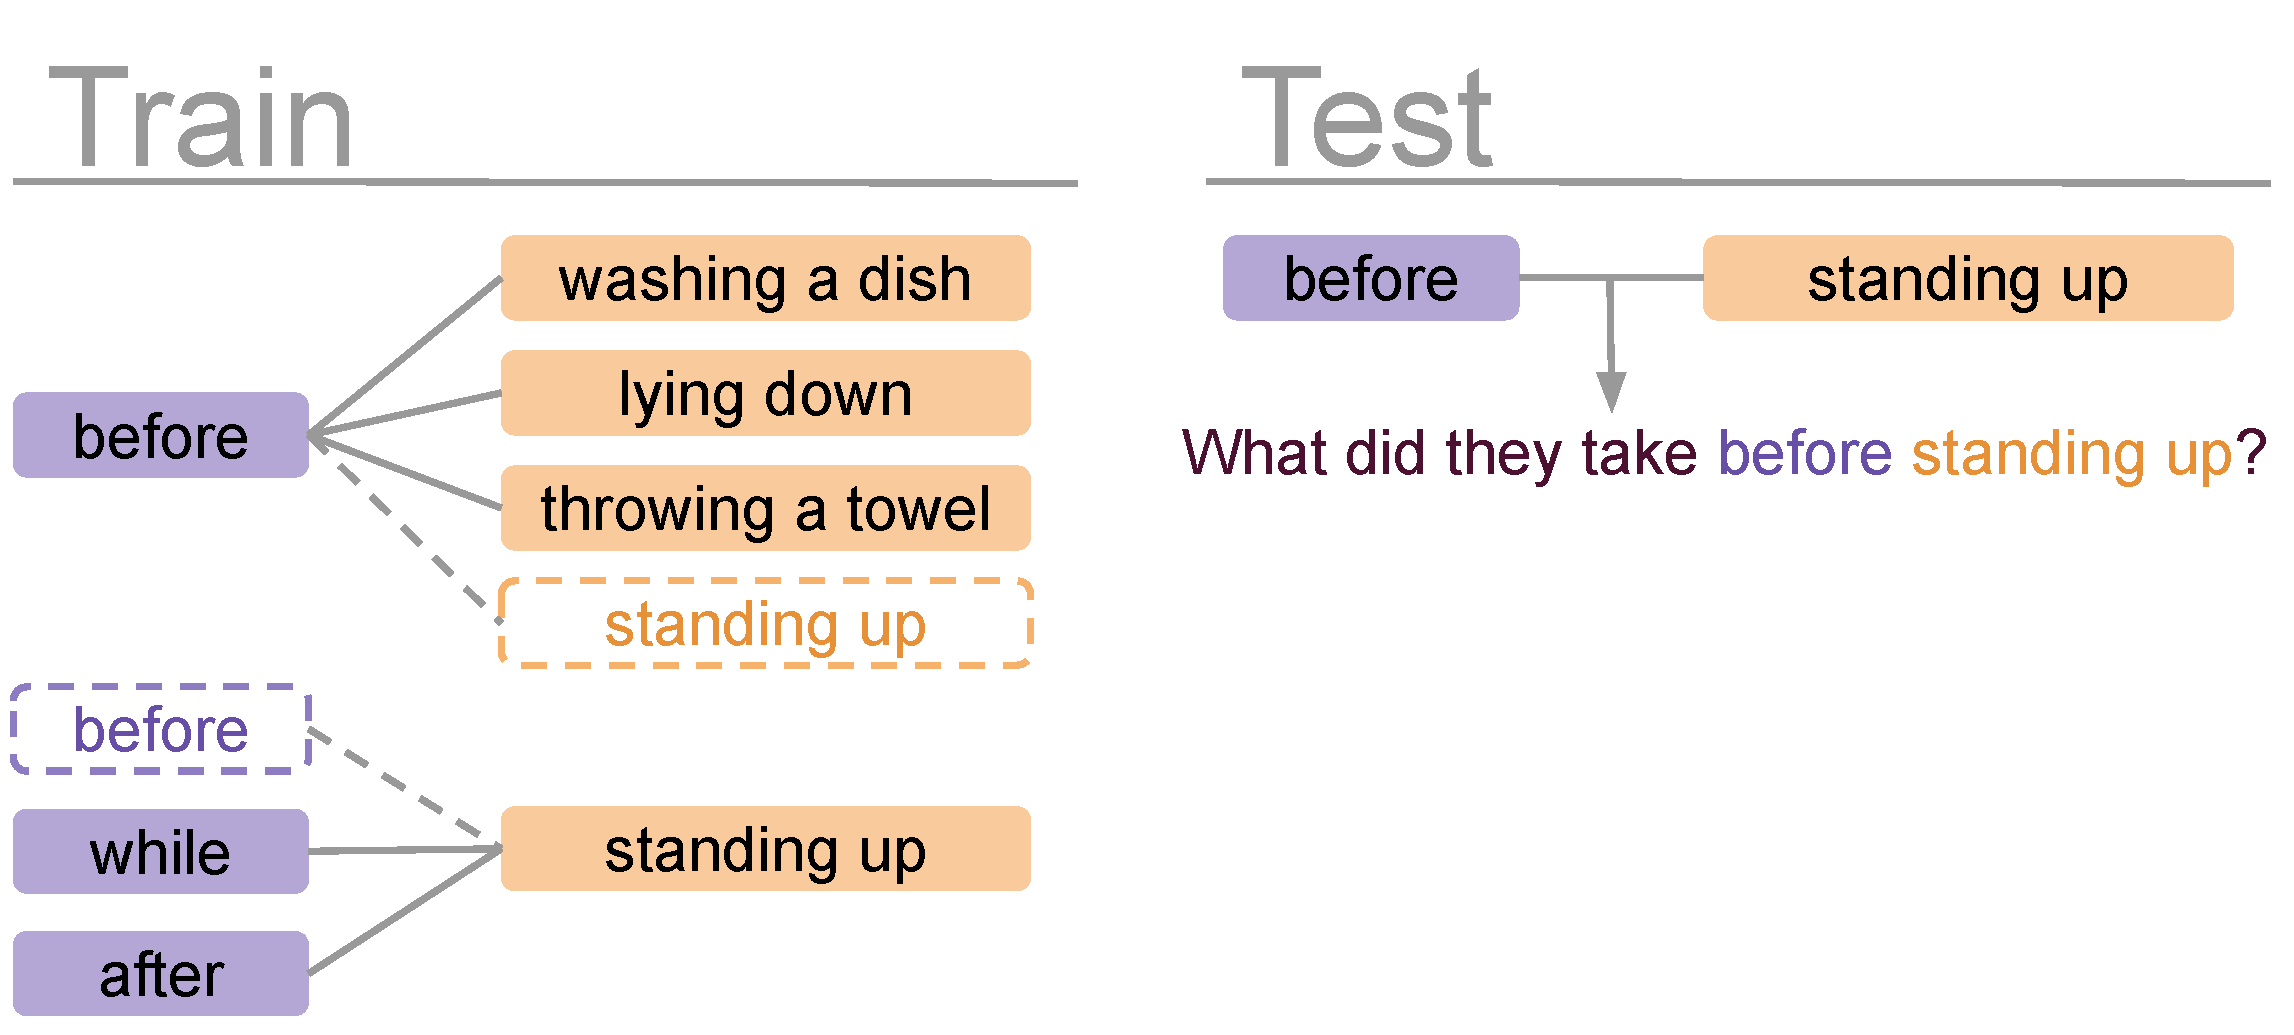
\includegraphics[width=0.95\linewidth]{figures/novel comp.pdf}
    \caption{We create a training and test split to measure a model's ability to generalize to novel compositions. In the training set, certain ideas like "before" and "standing up" are seen in many other contexts, but never combined with one another. In the test set, we look specifically at questions where these ideas are combined to see if the accuracy remains consistent with the validation set, implying that the model successfully generalized.}
    \label{fig:compo_fig}
\end{figure}



\subsection{Compositional metrics}

We also create metrics designed to measure compositional reasoning. These metrics ask if models, when trained on simpler or incomplete information, can successfully complete a more complex task.


\begin{figure*}[t]
\begin{center}
\begin{tabular}{ccccllllcc}
\multicolumn{1}{l}{}                                        & \multicolumn{1}{l}{} & \multicolumn{2}{c}{Random} & \multicolumn{2}{c}{PSAC}                           & \multicolumn{2}{c}{HME}                            & \multicolumn{2}{c}{HCRN} \\
\multicolumn{1}{l}{}                                        & \multicolumn{1}{l}{} & Val          & Test        & \multicolumn{1}{c}{Val} & \multicolumn{1}{c}{Test} & \multicolumn{1}{c}{Val} & \multicolumn{1}{c}{Test} & Val         & Test       \\
\rowcolor[HTML]{F3F3F3} 
\cellcolor[HTML]{F3F3F3}                                    & B                    & 35.39        & 38.88       &                         &                          &                         &                          & 41.06       & 34.26      \\
\rowcolor[HTML]{F3F3F3} 
\cellcolor[HTML]{F3F3F3}                                    & O                    & 31.14        & 33.41       &                         &                          &                         &                          & 33.33       & 21.57      \\
\rowcolor[HTML]{F3F3F3} 
\multirow{-3}{*}{\cellcolor[HTML]{F3F3F3}Novel Composition} & All                  & 34.29        & 37.47       &                         &                          &                         &                          & 37.01       & 28.22      \\
                                                            & B                    & 35.91        & 35.97       &                         &                          &                         &                          & 37.85       & 33.55      \\
                                                            & O                    & 23.53        & 25.66       &                         &                          &                         &                          & 31.02       & 28.58      \\
\multirow{-3}{*}{Video Lengths}                             & All                  & 32.70        & 33.29       &                         &                          &                         &                          & 34.35       & 31.05      \\
\rowcolor[HTML]{F3F3F3} 
\cellcolor[HTML]{F3F3F3}                                    & B                    & 40.52        & 26.20       &                         &                          &                         &                          & 47.63       & 26.20      \\
\rowcolor[HTML]{F3F3F3} 
\cellcolor[HTML]{F3F3F3}                                    & O                    & 24.57        & 18.60       &                         &                          &                         &                          & 31.58       & 23.59      \\
\rowcolor[HTML]{F3F3F3} 
\multirow{-3}{*}{\cellcolor[HTML]{F3F3F3}Steps Template}    & All                  & 36.33        & 36.50       &                         &                          &                         &                          & 38.95       & 27.61     
\end{tabular}
\end{center}
    \caption{We test the model on a variety of compositional reasoning skills. We check it's ability to generalize to novel compositions of ideas (Figure~\ref{fig:compo_fig}, from shorter videos to longer videos, and from simpler question structures to more complex questions structures.}
    \label{table:compo}
\end{figure*}


\begin{figure}[t]
\begin{center}
\resizebox{\linewidth}{!}{
\begin{tabular}{cccccc}
\multicolumn{1}{l}{}                             & \multicolumn{1}{l}{} & Random & PSAC & HME & HCRN  \\
\rowcolor[HTML]{F3F3F3} 
\cellcolor[HTML]{F3F3F3}                         & B                    & 39.81  &      &     & 39.19 \\
\rowcolor[HTML]{F3F3F3} 
\cellcolor[HTML]{F3F3F3}                         & O                    & 17.76  &      &     & 25.74 \\
\rowcolor[HTML]{F3F3F3} 
\multirow{-3}{*}{\cellcolor[HTML]{F3F3F3}Before} & All                  & 34.56  &      &     & 33.90 \\
                                                 & B                    & 49.93  &      &     & 29.07 \\
                                                 & O                    & 55.85  &      &     & 12.13 \\
\multirow{-3}{*}{First}                          & All                  & 51.62  &      &     & 20.90 \\
\rowcolor[HTML]{F3F3F3} 
\cellcolor[HTML]{F3F3F3}                         & B                    & 54.77  &      &     & 24.70 \\
\rowcolor[HTML]{F3F3F3} 
\cellcolor[HTML]{F3F3F3}                         & O                    & 38.52  &      &     & 20.38 \\
\rowcolor[HTML]{F3F3F3} 
\multirow{-3}{*}{\cellcolor[HTML]{F3F3F3}Longer} & All                  & 51.24  &      &     & 24.09 \\
                                                 & B                    & 25.15  &      &     & 1.50  \\
                                                 & O                    & 48.00  &      &     & 25.53 \\
\multirow{-3}{*}{Count}                          & All                  & 32.77  &      &     & 18.90 \\
\rowcolor[HTML]{F3F3F3} 
\cellcolor[HTML]{F3F3F3}                         & B                    & 52.45  &      &     & 33.20 \\
\rowcolor[HTML]{F3F3F3} 
\cellcolor[HTML]{F3F3F3}                         & O                    & 80.57  &      &     & 28.59 \\
\rowcolor[HTML]{F3F3F3} 
\multirow{-3}{*}{\cellcolor[HTML]{F3F3F3}ObjRel} & All                  & 58.48  &      &     & 31.43
\end{tabular}
}
\end{center}
   \caption{We check the model's ability to generalize to novel compositions combining the above concepts with an action, object, or relationship.}
\label{table:novel}
\end{figure}


\subsubsection{Novel Composition}

An important part of human reasoning is the ability to generalize concepts to novel compositions. One way to test this ability  is to train the model without a certain combination of phrases, then test it to see if it can still correctly reason about that phrase \cite{lake2018generalization}. For example, in the training set the model may never see the phrase "before standing up", but see both "before" and "standing up" in other contexts. Then, in the test set, we can test if it understands the  idea  of  ”before standing up”. We test combinations of ideas with questions asking the concenpts of before $<action>$, the first thing they $<$relation$>$, the $<$action$>$ they did for longer, the number of times an $<$action$>$ occurred, and several object-relation pairs. We are able to create such a training and testing split to judge these novel  compositions  because  we  have  knowledge  of what temporal localization, logical reasoning, and indirect tags are in each question.

As shown in Figure~\ref{table:compo}, the model's performance drops considerably from the validation set to the test set when it sees novel combinations of ideas. It especially struggles on questions asking about the number of times something occurred, and with open answer questions involving the concept of "first". 

\subsubsection{Indirect References}

This metric looks at questions that use only direct references to objects, relationships, and objects with no temporal localization. For models that get these questions correct, we ask them a series of other questions with the same base but using different levels of indirect references. \mgm{If i do it, say that we only add in indirect references } and sees if the model can still answer identical questions that use indirect references and temporal localizations. Add results here.

\mgm{maybe look at if it can answer questions where the whole indirect reference is masked}

\mgm{This will only be interesting if we fix indirects not affecting accuracy.}

\mgm{May want to make a separate table for this one too }

\subsubsection{Number of Compositional Steps}

In the previous metric, the model has seen both levels of complexity in training. In this metric, we look at if the model is able to generalize to more complex compositional structures after training on simple compositional structures \cite{lake2018generalization}. This metric measures compositional complexity through the number of "steps" each question has, which represents the number of reasoning operations needed to answer it. For each template, we find a the number of steps such that at least 50\% of the questions are at that number of steps or fewer. Then, in the training set, we train only on questions that are less than or equal to that marker. In the test set, we only test on questions that are greater than that marker. The marker is high enough that some indirect references are seen in the training set, however in the test set the model must make much more complex combinations and reasoning feats than before. For this metric, we balance the distribution of questions such that for every question in which a temporal localization phrase does not change the answer, there is at least one where it does.

The model's accuracy drops from above random, to at random for binary questions, and decreases ts lead above random for open answer questions.


\subsubsection{Length of video}

Some video models are better at shorter or longer videos. Many existing video datasets are on short videos and many models are inflexible with video length \cite{le2020hierarchical}. This metric tests if models trained on short videos can generalize to being tested on long videos. HCRN was made specifically to be more flexible with video length, and its accuracy only drops slightly when tested on the longer videos.


\section{Conclusion and Limitations}

Coherent Idea: 

\mgm{A lot of separate ideas here, need to find a coherent flow}

Compared to other VideoQA datasets we measure a wider variety of spatio-temporal topics. We also measure compositional reasoning on non-synthetic videos. 

Shortcomings and successes of existing systems (once get results)

Limitation of this generation model to the annotations. Although we did a lot of edits to create high quality questions, some annotation errors will be built into the 

Challenges with having actions as open answers because action segmentation is so uncertain.

Future work could expand to other types of answers, like time stamps, bounding boxes, and lists. Furthermore, future work could expand out from the limited set of objects, relationships, and actions seen in Charades Videos. 

{\small
\bibliographystyle{ieee_fullname}
\bibliography{references}
}

\end{document}
